



\section{CHAPTER 10}


\subsubsection{
\subsection{Section 10.1}}

*************
1.
*************
<answer><p> The number of trees are: (a) 1, (b) 3, and (c) 16.  The trees that connect \(V_c\) are:

\begin{doublespace}
\noindent\(\)
\end{doublespace}

</p></answer>


*************
3
*************
<answer><p>  \textit{ Hint:} Use induction on \(\left| E\right|\).

</p></answer>


*************
5
*************
<answer><p> (a) Assume that \((V,E)\) is a tree with \(\left| V\right| \geq 2\), and all but possibly one vertex in <m>V</m> has degree two or more.



\(2\left| E\right| =\sum \text{\textit{$\deg  (v)$}}\text{\textit{$\geq $}}\text{\textit{$2\left| V\right| $}}\text{\textit{$-$}}1\\
\\
\quad v\in V\\
\\
\text{or}\text{  }\left| E\right| \geq \left| V\right| -\frac{1}{2}\Rightarrow \left| E\right| \geq \left| V\right| \Rightarrow (V,E) \text{is} \text{not}
a \text{tree}.\)

</p></li>
<li><p> The proof of this part is similar to part a in that we get \(2\left| E\right| \geq 2\left| V\right| -1\), since a tree that is not a chain has
a vertex with degree three or more.




\subsection{Section 10.2}

*************
1.
*************
<answer><p> It might not be most economical with respect to Objective 1. You should be able to find an example to illustrate this claim. The new system can
always be made most economical with respect to Objective 2 if the old system were designed with that objective in mind.
</p></answer>


*************
3
*************
<answer><ol><li><p>Edges in one solution are: \(\{8,7\},\{8,9\},\{8,13\},\{7,6\},\{9,4\},\{13,12\},\{13,14\},\{6,11\},\{6,1\},\{1,2\},\{4,3\},\{4,5\},\{14,15\},
\textrm{ and } \{5,10\}\)</p></li>
<li><p> Vertices 8 and 9 are at the center of the graph. Starting from vertex 8, a minimum diameter spanning tree is \(\{\{8, 3\}, \{8, 7\}, \{8, 13\},
\{8, 14\}, \{8, 9\}, \{3, 2\}, \{3, 4\}, \{7, 6\}, \{13, 12\}, \{13, 19\}, \{14, 15\}, \{9, 16\}, \{9, 10\}, \{6, 1\}, \{12, 18\}, \{16, 20\}, \{16,
17\}, \{10, 11\}, \{20, 21\}, \{11, 5\}\}. \text{The} \text{diameter} \text{of} \text{the} \text{tree} \text{is} 7.\)
</p></li></ol></answer>




\subsection{Section 10.3}

*************
1.
*************
<answer><p> Locate any simple path of length \textit{ d }and locate the vertex in position \(\lceil d/2\rceil\)on the path. The tree rooted at that vertex
will have a depth of \(\lceil d/2\rceil\), which is minimal.

</p></answer>


*************
3
*************
<answer><p>

\begin{doublespace}
\noindent\(\)
\end{doublespace}








\subsection{Section 10.4}

*************
1.
*************
<answer><p>

\begin{doublespace}
\noindent\(\)
\end{doublespace}

\begin{doublespace}
\noindent\(\)
\end{doublespace}





</p></answer>


*************
3
*************
<answer><p>  \(\begin{array}{cccc}
   &amp; \text{Preorder}  &amp; \text{Inorder}\text{   } &amp; \text{Postorder} \\
 (a)\text{   } &amp; \cdot a+\text{\textit{bc}}\text{\textit{      }} &amp; a\cdot b+c\text{   } &amp; \text{\textit{abc}}+\cdot \text{     } \\
 (b)\text{   } &amp; +\cdot \text{\textit{abc}}\text{\textit{      }} &amp; a\cdot b+c\text{    } &amp; \text{\textit{ab}}\cdot c+\text{     } \\
 (c)\text{   } &amp; +\cdot \text{\textit{ab}}\cdot \text{\textit{ac}}\text{\textit{$ $}} &amp; a\cdot b+a\cdot c\text{  } &amp; \text{\textit{ab}}\cdot \text{\textit{ac}}\cdot
+  \\
\end{array}\)

</p></answer>


*************
5
*************
<answer><p>

\begin{doublespace}
\noindent\(\)
\end{doublespace}

</p></answer>


*************
7
*************
<answer><p> Solution $\#$1:



Basis:A binary tree consisting of a single vertex, which is a leaf, satisfies the equation \(\text{leaves} = \text{internal} \text{vertices}
+ 1\),



Induction:Assume that for some \(k\geq 1\), all full binary trees with <m>k</m> or fewer vertices have one more leaf than internal vertices.
Now consider any full binary tree with \(k+1\) vertices. Let \(T_A\text{and} T_B\) be the left and right subtrees of the tree which, by the definition
of a full binary tree, must both be full. If \(i_A\text{and} i_B\) are the numbers of internal vertices in \(T_A\text{and} T_B\), and \(j_A\text{and}
j_B\) are the numbers of leaves, then \(j_A=i_A+1 \text{and} j_B=i_B+1\). Therefore, in the whole tree, the number of leaves \(=j_A+j_B\\
\\
=\left(i_A+1\right)+\left(i_B+1\right)\\
\\
=\left(i_A+i_B+1\right)+1\\
\\
=(\text{number} \text{of} \text{internal} \text{vertices})+1\)



Solution $\#$2: Imagine building a full binary tree starting with a single vertex. By continuing to add leaves in pairs so that the tree
stays full, we can build any full binary tree. Our starting tree satisfies the condition that the number of leaves \((1)\) is one more than the number
of internal vertices \((0)\). By adding a pair of leaves to a full binary tree, an old leaf becomes an internal vertex, increasing the number of
internal vertices by one. Although we lose a leaf, the two added leaves create a net increase of one leaf. Therefore, the desired equality is maintained.




\subsection{Supplementary Exercises$---$Chapter 10}

*************
1.
*************
<answer><p> Each of the \(n-1\) edges of a tree contributes to the degrees of two vertices. Therefore the sum of all degrees of vertices in an <m>n</m>
vertex tree is \(2(n-1)=2n-2\).

</p></answer>


*************
3
*************
<answer><p> (a) \(G_2\text{is} \text{graceful}: v_1=1, v_2+2, v_3=4\\
\\
G_4\text{is} \text{graceful}: v_1=2, v_2=1, v_3=3, v_4=4\)

</p></li>
<li><p> Starting at either end of the chain label the first vertex \(S(1)=1\) and the \((k+1)\text{st} \text{vertex}, k\geq 1, S(k+1)=S(k)+k\). The edge
connecting the \(k\text{th}\) and \((k+1)\text{st}\) vertex is the \(\text{kth}\) edge and since \((S(k+1)-s(k))=k\), the chain is graceful. The
closed form expression for \(S(k) \text{is} 1+\left(k\left(k-\frac{1}{2}\right)\right)\).

</p></answer>


*************
5
*************
<answer><p> First, \(\{3,6\}\) is added to the edge set, then \(\{1,2\} \text{and} \{3,4\}\). Then \(\{4,6\}\) is rejected since it would complete a  cycle.
This can be seen from the forest.

\begin{doublespace}
\noindent\(\)
\end{doublespace}



Vertices 4 and 6 have the same root in this tree; hence \(\{4,6\}\) is rejected. \(\{1,5\} \text{and} \{2,3\}\) are the final edges that complete
the minimal spanning tree. Notice that \(\{4,6\}\) could have been the second edge selected. In that case, \(\{3,4\}\) would be rejected.

</p></answer>


*************
7
*************
<answer><p> The depth of the tree is four.

\begin{doublespace}
\noindent\(\)
\end{doublespace}

</p></answer>


*************
9
*************
<answer><p><ol label="a">
<li><p>

\begin{doublespace}
\noindent\(\)
\end{doublespace}

</p></li>
<li><p>   \(\text{\textit{aa}}\cdot 2a\cdot b\cdot +b+\) is the postorder traversal of the tree. This is also the postfix version of the original expression.


\section{CHAPTER 11}


\subsection{Section 11.1}

*************
1.
*************
<answer><p> (a) Commutative, and associative. Notice that zero is the identity for addition, but it is not a positive integer.)

</p></li>
<li><p> Commutative, associative, and has an  identity (1)

</p></li>
<li><p> Commutative, associative, has an identity (1), and is idempotent

</p></li>
<li><p> Commutative, associative, and idempotent

</p></li>
<li><p>  None. Note:   \(2 @ (3 @ 3) = 512 \\
\\
 (2 @ 3) @ 3 = 64\)



        and while \(a @ 1 = a\), \(1 @ a = 1\).

</p></answer>


*************
3
*************
<answer><p>  \(a, b \in  A \cap  B\text{  }\Rightarrow \text{  }a, b \in  A\text{  }\text{by} \text{the} \text{definition} \text{of} \text{intersection}\\
\\
\quad \quad \quad \Rightarrow  a*b\in A\text{   }\text{by} \text{the} \text{closure} \text{of} A \text{with} \text{respect} \text{to} *\) 



     Similarly, \(a, b \in  A \cap B\Rightarrow  a*b\in B\). Therefore, \(a * b \in  A \cap  B\).



The set of positive integers is closed under addition, and so is the set of negative integers, but \(1 + -1 - 0\). Therefore, their union, the nonzero
integers, is not closed under addition.</p></answer>


*************
5
*************
<answer><p> Let $\mathbb{N}$ be the set of all nonnegative integers (the natural numbers).

</p></li>
<li><p> \(*\) is commutative since \(\left| a-b\right| =\left| b-a\right|\) for all \(a, b \in  \mathbb{N}\)

</p></li>
<li><p> \(*\) is not associative. Take \(a = 1\), \(b = 2\), and \(c = 3\), then



\((a * b) * c =\left| \left| 1-2\right| -3\right| =2\) , and



\(a * (b * c) = \left| 1-\left| 2-3\right| \right| = 0\).

</p></li>
<li><p> Zero is the identity for \(*\) on $\mathbb{N}$, since



\(a*0=\left| a+0\right|  = a = \left| 0-a\right| = 0 * a.\)

</p></li>
<li><p>  \(a^{-1}=a\)  for each a $\in $ $\mathbb{N}$, since



\(a * a=\left| a-a\right|  = 0\).

</p></li>
<li><p> \(*\) is not idempotent, since, for \(a\neq 0\),



$\quad \quad $\(a * a =0 \neq a\).


\subsection{Section 11.2}

*************
1.
*************
<answer><p> The terms {``}generic{''} and {``}trade{''} for prescription drugs are analogous to {``}generic{''} and {``}concrete{''} algebraic systems. {
}Generic aspirin, for example, has no name, whereas Bayer, Tylenol, Bufferin, and Anacin are all trade or specific types of aspirins. The same can
be said of a generic group \([G, *]\) where <m>G</m> is a nonempty set and \(*\) is a binary operation on \(G\), When examples of typical domain
elements can be given along with descriptions of how operations act on them, such as $\mathbb{Q}$* or \(M_{2\times 2}(\mathbb{R})\), then the system
is concrete (has a specific name, as with the aspirin). Generic is a way to describe a general algebraic system, whereas a concrete system has a
name or symbols making it distinguishable from other systems.

</p></answer>


*************
3
*************
<answer><p>  b, d, e, and f.

</p></answer>


*************
5
*************
<answer><p> (a)  \(\left(
\begin{array}{cc}
 1 &amp; 0 \\
 0 &amp; 1 \\
\end{array}
\right)\), \(\left(
\begin{array}{cc}
 0 &amp; 1 \\
 1 &amp; 0 \\
\end{array}
\right)\),  abelian



    (b)     \(\begin{array}{c|c}
   &amp; 
\begin{array}{cccccc}
 I &amp; R_1 &amp; R_2 &amp; F_1 &amp; F_2 &amp; F_3 \\
\end{array}
 \\
\hline
 
\begin{array}{c}
 I \\
 R_1 \\
 R_2 \\
 F_1 \\
 F_2 \\
 F_3 \\
\end{array}
 &amp; 
\begin{array}{cccccc}
 I &amp; R_1 &amp; R_2 &amp; F_1 &amp; F_2 &amp; F_3 \\
 R_1 &amp; R_2 &amp; I &amp; F_2 &amp; F_3 &amp; F_1 \\
 R_2 &amp; I &amp; R_1 &amp; F_3 &amp; F_1 &amp; F_2 \\
 F_1 &amp; F &amp; F_2 &amp; I &amp; R_2 &amp; R_1 \\
 F_2 &amp; F_1 &amp; F_3 &amp; R_1 &amp; I &amp; R_2 \\
 F_3 &amp; F_2 &amp; F_1 &amp; R_2 &amp; R_1 &amp; I \\
\end{array}
 \\
\end{array}\)



This group is non-abelian since, for example,  \(F_1F_2=R_2\) and \(F_2F_1=R_2\).



 (c) 4! = 24, n!</p></answer>


*************
7
*************
<answer><p>  The identity is <m>e</m>.   \(a*b = c\), \(a*c= b\),  \(b*c = a\), and \([V, *]\) is abelian. (This group is commonly called the Klein-4
group.)


\subsection{Section 11.3}

*************
1.
*************
<answer><p> (a)  <m>f</m> is injective: \(\text{       }f(x) = f(y) \Rightarrow  a * x = a * y \quad \quad \Rightarrow  x = y\text{      }(\text{by}
\text{left} \text{cancellation})\)



         \textit{ f }is surjective:  For all <m>b</m>,   \(f(x) = b\) has the solution \(a^{-1}*b\).



    (b) Functions of the form \(f(x)\text{  }= a + x\), where <m>a</m> is any integer, are bijections

</p></answer>


*************
3
*************
<answer><p>  Basis: (\(n = 2\))   \(\left(a_1*a_2\right){}^{-1}= a_2{}^{-1}*a_1{}^{-1}\) by Theorem 11.3.4.



Induction: Assume that for some \(n \geq  2\),



$\quad \quad $\(\left(a_1*a_2*\cdots *a_n\right){}^{-1}=a_n{}^{-1}*\cdots * a_2{}^{-1}*a_1{}^{-1}\)



We must show that



$\quad \quad $\(\left(a_1*a_2*\cdots *a_n*a_{n+1}\right){}^{-1}=a_{n+1}{}^{-1}*a_n{}^{-1}*\cdots * a_2{}^{-1}*a_1{}^{-1}\)



This can be accomplished as follows:



\(\text{            }\left(a_1*a_2*\cdots *a_n*a_{n+1}\right){}^{-1}=\left(\left(a_1*a_2*\cdots *a_n\right)*a_{n+1}\right){}^{-1}\text{ 
 }\text{by} \text{the} \text{associative} \text{law}\quad \quad \quad \quad =a_{n+1}{}^{-1}*\left(a_1*a_2*\cdots *a_n\right){}^{-1}\text{   }\text{by}
\text{the} \text{basis}\quad \quad \quad \quad =a_{n+1}{}^{-1}*\left(a_n{}^{-1}*\cdots * a_2{}^{-1}*a_1{}^{-1}\right)\text{  }\text{by} \text{the}
\text{induction} \text{hypothesis}\quad \quad \quad \quad = a_{n+1}{}^{-1}*a_n{}^{-1}*\cdots * a_2{}^{-1}*a_1{}^{-1} \text{by} \text{the} \text{associative}
\text{law}\text{   }\blacksquare\)

</p></answer>


*************
5
*************
<answer><p> (a) Let \(p(n)\) be, where <m>a</m> is any element of group \([G; *]\). First we will prove that \(p(n)\) is true for all \(n \geq  0\).



First, we would need to prove a lemma that we leave to the reader, that if \(n\geq 0\), and <m>a</m> is any group element, \(a*a^n=a^n*a\). 



Basis: If \(n = 0\), Using the definition of the zero exponent,  \(\left(a ^0\right) ^{-1} = e^{-1} = e\),  while \(\left(a^{-1}\right)^0= e\).
Therefore, \(p(0)\) is true.



Induction: Assume that for some \(n \geq  0\), \(p(n\)) is true.



\(\text{               }\left(a^{n+1}\right)^{-1}= \left(a^n*a\right)^{-1}\text{   }\text{by} \text{the} \text{definition} \text{of} \text{exponentiation}\quad
\quad =a^{-1}*\left(a^n\right)^{-1}\text{     }\text{by} \text{Theorem}\text{  }11.3\cdot 4\quad \quad = a^{-1}*\left(a^{-1}\right)^n\text{   }\text{by}
\text{the} \text{induction} \text{hypothesis}\quad \quad = \left(a^{-1}\right)^{n+1} \text{by} \text{the} \text{lemma}\)



If <m>n</m> is negative, then \(-n\) is positive and



$\quad \quad $\(\text{   }a^{-n}= \left(\left(\left(a^{-1}\right)^{-1}\right)^{-n} \right)\text{  }\quad =\left(a^{-1}\right)^{-(-n)}\text{  }\text{since}
\text{the} \text{property} \text{is} \text{true} \text{for}\text{  }\text{positive} \text{numbers}\quad =\left(a^{-1}\right)^n\)

</p></li>
<li><p> For \(m > 1\), let \(p(m)\) be \(a^{n+m}=a^n*a^m\) for all \(n\geq 1\). The basis for this proof follows directly from the basis for the definition
of exponentiation.



Induction: Assume that for some \(m > 1\), \(p(m)\) is true. Then



\(\text{                }a^{n+(m+1)}= a^{(n+m)+1}\text{   }\text{by} \text{the} \text{associativity} \text{of} \text{integer} \text{addition}\quad
\quad =a^{n+m}*a^1\text{  }\text{by} \text{the} \text{definition} \text{of} \text{exponentiation}\quad \quad =\left(a^n*a^m\right)*a^1\text{  }\text{by}
\text{the} \text{induction} \text{hypothesis}\quad \quad = a^n*\left(a^m*a^1\right)\text{   }\text{by} \text{associativity}\quad \quad = a^n*a^{m+1}\text{
 }\text{by} \text{the} \text{definition} \text{of} \text{exponentiation}\)

</p></li>
<li><p> Let \(p(m)\)be \(\left(a^n\right)^m= a^{n m}\) for all integers <m>n</m>.



Basis: \(\left(a^m\right)^0= e\) and \(a^{m\cdot 0}=a^0= e\) therefore, \(p(0)\) is true.



Induction; Assume that \(p(m)\) is true for some \(m >\)0,



\(\quad \left(a^n\right)^{m+1}=\left(a^n\right)^m*a^n\text{    }\text{definition} \text{of} \text{exponentiation}\quad \quad =a^{n m}*a^n\text{
      }\text{by} \text{the} \text{induction} \text{hypothesis}\quad \quad =a^{n m + n}\text{          }\text{by} \text{part} (a) \text{of} \text{this}
\text{problem}\quad \quad =a^{n(m+1)}\text{          }\)



Finally, if <m>m</m> is negative, we can verify that \(\left(a^n\right)^m= a^{n m}\) using many of the same steps as the proof of part (a).


\subsection{Section 11.4}

*************
1.
*************
<answer><p><ol label="a">
<li><p> 2 (b) 5 $\quad \quad $(c) 0



   </p></li>
<li><p> 0 (e) 2 $\quad \quad $(f) 2 



   </p></li>
<li><p> 1 (h) 3</p></answer>


*************
3
*************
<answer><p><ol label="a">
<li><p> 1 (b) 1 $\quad \quad $(c) \(m(4) = r(4)\), where \(m = 11 q + r\), \(0 \leq  r < 11\) .

</p></answer>


*************
5
*************
<answer><p> Since the solutions, if they exist, must come from \(\mathbb{Z}_2\) , substitution is the easiest approach.



(a) 1 is the only solution, since  \(1^2+_21=0\)   and  \(0^2+_21=1\)



(b) No solutions, since \(0^2+_20+_21=1\), and  \(1^2+_21+_21=1\)

</p></answer>


*************
7
*************
<answer><p> Hint: Prove by induction on <m>m</m> that you can divide any positive integer into <m>m</m>, That is, let \(p(m)\) be $\texttt{"}$For all
<m>n</m> greater than zero, there exist unique integers <m>q</m> and <m>r</m> such that. . . .$\texttt{"}$ In the induction step, divide
<m>n</m> into \textit{ m - n}.


\subsection{Section 11.5}

*************
1.
*************
<answer><p>   a and c

</p></answer>


*************
3
*************
<answer><p>   \(\left\{I,R_1,R_2\right\}\), \(\left\{I,F_1\right\}\), \(\left\{I,F_2\right\}\), and \(\left\{I,F_3\right\}\) are all the proper subgroups
of \(R_3\).

</p></answer>


*************
5
*************
<answer><p>  <ol label="a">
<li><p> \(\langle 1\rangle  = \langle 5\rangle  = \mathbb{Z}_6\)



\(\quad\)\(\langle 2\rangle \text = \langle 4\rangle  = \{2, 4, 0\}\)



\(\langle 3\rangle \text = \{3, 0\}\)



\(\langle 0\rangle  = \{0\}\)



     </p></li>
<li><p> \(\langle 1\rangle  = \langle 5\rangle  = \langle 7\rangle  = \langle 11\rangle  =\mathbb{Z}_{12}\)



\(\langle 2\rangle \text = \langle 10\rangle  = \{2, 4, 6, 8, 10, 0\}\)



\(\langle 3\rangle \text = \langle 9\rangle  = \{3, 6, 9, 0\}\)



\(\langle 4\rangle \text = \langle  8 \rangle  = \{ 4 , 8, 0\}\)



\(\langle 6\rangle  = \{6, 0\}\) 



\(\langle 0\rangle  = \{0\}\)



   </p></li>
<li><p>   \(\langle 1\rangle  = \langle  3\rangle  = \langle  5 \rangle  = \langle 7\rangle  = \mathbb{Z}_8\)



\(\langle 2\rangle  = \langle 6\rangle  = \{2, 4, 6, 0\}\) 



\(\langle 4\rangle  = \{4, 0\}\)



\(\langle 0\rangle  = \{0\}\)

\begin{doublespace}
\noindent\(\begin{array}{lll}
  &amp;  &amp;  \\
\end{array}\)
\end{doublespace}

</p></li>
<li><p> Based on the ordering diagrams in parts a through c, we would expect to see an ordering diagram similar to the one for divides on \(\{1, 2, 3,
4, 6, 8, 12, 24\}\) (the divisors of 24) if we were to examine the subgroups of \(\mathbb{Z}_{24}\). This is indeed the case.

</p></answer>


*************
7
*************
<answer><p> Assume that <m>H</m> and <m>K</m> are subgroups of group <m>G</m>, and that, as in Figure 11.5.1, there are elements \(x \in  H --- K\)
and \(y \in  K --- H\). Consider the product \(x * y\). Where could it be placed in the Venn diagram? If we can prove that it must lie in the outer
region, \(H^c\cap K^c=(H\cup K)^c\), then we have proven that \(H \cup  K\) is not closed under \(*\) and can{'}t be a subgroup of <m>G</m>, Assume
that  \(x*y\in H\).  Since \(x\) is in \textit{ H,} \(x^{-1}\) is in <m>H</m> and so by closure



\(x^{-1}*(x * y )= y \in H\)



which is a contradiction.   Similarly, \(x*y \notin K\).  $\blacksquare $ 



One way to interpret this theorem is that no group is the union of two groups.


\subsection{Section 11.6}

*************
1.
*************
<answer><p> Table of \(\mathbb{Z}_2\times  \mathbb{Z}_3\) :

\begin{doublespace}
\noindent\(\begin{array}{cc}
 \text{} &amp;  \\
  &amp;  \\
\end{array}\)
\end{doublespace}



The only two proper subgroups are \(\{(0, 0), (1, 0)\}\) and \(\{(0, 0), (0, 1), (0, 2)\}\)</p></answer>


*************
3
*************
<answer><p> (a) (i) \(a + b\text{  }\text{could} \text{be}\text{  }(1, 0) \text{or} (0, 1)\). 



(ii)  \(a + b = (1, 1)\).

</p></li>
<li><p> (i) \(a + b = \text{could} \text{be}\text{  }(1, 0, 0), (0, 1, 0), \text{or}\text{  }(0, 0, 1)\). 



(ii) \(a + b = (1, 1, 1)\).

</p></li>
<li><p> (i) \(a + b\) has exactly one 1.



(ii) \(a + b\) has all \(1's\).

</p></answer>


*************
5
*************
<answer><p> </p></li>
<li><p>  No,  0 is not an element of \(\mathbb{Z} \times \mathbb{Z}\).  </p></li>
<li><p> Yes. </p></li>
<li><p> No, (0, 0) is not an element of this set.



     </p></li>
<li><p> No, the set is not closed: \((1, 1) + (2, 4) = (3, 5)\) and \((3, 5)\) is not in the set. </p></li>
<li><p> Yes.


\subsection{Section 11.7}

*************
1.
*************
<answer><p> (a) Yes, \(f(n, x) = (x, n)\) for \((n, x) \in  \mathbb{Z} \times  \mathbb{R}\) is an isomorphism. 

</p></li>
<li><p> No, \(\mathbb{Z}_2\times  \mathbb{Z}\) has a finite proper subgroup while \(\mathbb{Z} \times  \mathbb{Z}\) does not.

</p></li>
<li><p> No. 

</p></li>
<li><p> Yes.

</p></li>
<li><p>  No. 

</p></li>
<li><p> Yes,  one isomorphism is defined by \(f\left(a_1, a_2,a_3,a_4\right)=\left(
\begin{array}{cc}
 a_1 &amp; a_2 \\
 a_3 &amp; a_4 \\
\end{array}
\right)\). 

</p></li>
<li><p> Yes, one isomorphism is defined by \(f\left(a_1,a_2\right)=\left(a_1,10^{a_2}\right)\). 

</p></li>
<li><p> Yes. 

</p></li>
<li><p> Yes   \(f(k) = k(1,1)\).</p></answer>


*************
3
*************
<answer><p>  Consider 3 groups \(G_1\), \(G_2\), and \(G_3\) with operations \(*, \diamond , \text{and} \square\), respectively.. We want to show that if
\(G_1\) is isomorphic to \(G_2\) , and if \(G_2\) is isomorphic to \(G_3\) , then \(G_1\) is isomorphic to \(G_3\).



\(G_1 \text{isomorphic} \text{to} G_2\Rightarrow  \text{there} \text{exists} \text{an} \text{isomorphism} f:G_1\to G_2\) 



\(G_2 \text{isomorphic} \text{to} G_3\Rightarrow  \text{there} \text{exists} \text{an} \text{isomorphism} g:G_2\to G_3\) 



If we compose <m>g</m> with <m>f</m>, we get the function \(g\circ f:G_1\to G_3\),  By Theorems 7.3.2 and 7.3.3, \(g\circ f\) is a bijection,
and if \(a,b\in G_1\),



\((g\circ f)(a*b)=g(f(a*b))\\
\\
\quad \quad =g(f(a)\diamond f(b))\text{  }\text{since} f \text{is} \text{an} \text{isomorphism}\\
\\
\quad \quad =g(f(a))\square g(f(b)) \text{since} g \text{is} \text{an} \text{isomorphism}\\
\\
\quad \quad =(g\circ f)(a) * (g\circ f)(b)\)



Therefore, \(g\circ f\) is an isomorphism from \(G_1\) into \(G_3\) , proving that {``}is isomorphic to$\texttt{"}$ is transitive.

</p></answer>


*************
5
*************
<answer><p>  \(\mathbb{Z}_8\), \(\mathbb{Z}_2\times  \mathbb{Z}_4\) , and \(\mathbb{Z}_2{}^3\)$|$. One other is the fourth dihedral group, introduced in
Section 15.3.</p></answer>


*************
7
*************
<answer><p> Let <m>G</m> be an infinite cyclic group generated by <m>a</m>. Then, using multiplicative notation,  \(G=\left\{\left.a^n\right| n\in
\mathbb{Z}\right\}\).



The map \(T: G ---> \mathbb{Z}\) defined by \(T\left(a^n\right)=n\) is an isomorphism. This is indeed a function, since \(a^n=a^m\) implies \(n =m\).
Otherwise, <m>a</m> would have a finite order and would not generate <m>G</m>.



(a)  T is one-to-one, since \(T\left(a^n\right) = T\left(a^m\right)\) implies \(n = m\), so \(a^n= a^m\).



(b)  T is onto, since for any \(n\in \mathbb{Z}\), \(T\left(a^n\right) = n\).



(c)   \(\text{          }T\left(a^n*a^m \right) = T\left(a^{n+m}\right)\quad \quad =n + m\quad \quad =T\left(a^n\right)+T\left(a^m\right)\)


\subsection{Supplementary Exercises$---$Chapter 11}

*************
1.
*************
<answer><p> (a) With respect to <m>V</m> under +, the identity is <m>a</m>; and \(-a=a\),  \(-b=c\), and \(-c=b\).

</p></li>
<li><p> With respect to <m>V</m> under \(\cdot\), the identity is <m>b</m>. Inverses:  \(b^{-1}=b\), \(c^{-1}=c\), and <m>a</m> has no inverse,

</p></li>
<li><p> \(\cdot\) is distributive over + since \(x \cdot  (y + z) = x \cdot y + x\cdot  z\) for each of the 27 ways that the variables <m>x</m>, \textit{
y}, and <m>z</m> can be assigned values from <m>V</m>.  However, + is not distributive over \(\cdot\) since \(b + (a \cdot c) = b\), while
\((b + a) \cdot  (b + c) = a\),

</p></answer>


*************
3
*************
<answer><p>  By Theorem 7.3.4 every bijection has an inverse, so \(\circ\) has the inverse property on <m>S</m>. If \(f \in  S\),



 \(f\circ f^{-1}= f^{-1}\circ f=i\text{    }\Rightarrow \text{  }f \text{inverts} f^{-1},\text{   }\text{or}\text{     }\left(f^{-1}\right)^{-1}=
f.\)



Therefore, inversion of functions has the involution property.

</p></answer>


*************
5
*************
<answer><p> If <m>a</m> and <m>b</m> are odd integers, \(a = 2j + 1\) and \(b = 2k + 1\) for \(j, k \in  \mathbb{Z}\). \(a b = (2j + 1)(2k + 1) = 2(2j
k + j + k) + 1\), which is an odd integer. Since 1 is odd and \(1 + 1\) is even, the odds are not closed under addition, The even integers are closed
under both addition and multiplication. If <m>a</m> and <m>b</m> are even, \(a = 2j\) and \(b = 2k\) for some \(j, k \in  \mathbb{Z}\), \(a
+ b = 2j + 2k = 2(j + k)\), which is even, and \(a b = (2j)(2k) = 2(2j k)\), which is also even.

</p></answer>


*************
7
*************
<answer><p>  That \(\text{GL}(2,\mathbb{R})\) is a group follows from laws of matrix algebra. In addition to being associative, matrix multiplication on
two-by-two matrices has an identity <m>I</m>, and if \(A \in  \text{GL} (2,\mathbb{R})\), it has an inverse by the definition of \(\text{GL} (2,\mathbb{R})\).
The inverse of A is in GL(2,$\mathbb{R}$) since it has an inverse: \(\left(A^{-1}\right)^{-1} = A\).

</p></answer>


*************
9
*************
<answer><p> If \(a, b, c \in  \mathbb{R}\),



 \(\text{          }(a * b) * c = (a + b + 5) * c\quad \quad =a+b+5+c+5\quad \quad =a+b+c+10\)



 \(a * (b * c)\) is also equal to \(a+b+c+10\), and so \(*\) is associative. To find the identity we solve \(a * e =\)a for \textit{ e:}



\(a * e = a\text{   }\Rightarrow \text{  }a + e + 5 = a\text{   }\Rightarrow \text{  }e = ---5\).



If <m>a</m> is a real number, the inverse of <m>a</m> is determined by solving the equation \(a * x=-5\);



\(a*x=-5\text{  }\Rightarrow  a + x + 5 = -5\text{  }\Rightarrow  x = -a-10\)



Since <m>a</m> is real, \(-a-10\) is real, and so \(*\) has the inverse property.</p></answer>


*************
11
*************
<answer><p> By Supplementary Exercise 2 of this chapter, the identity for \(*\) is 2 and \(*\) is associative. All that is left to show is that * has the
inverse property. If \(a \in  \mathbb{Q}^+\)  , \(a * x = 2 \Rightarrow  x = \frac{4}{a}\); hence  \(a^{-1}= \frac{4}{a}\), which is also a positive
rational number.</p></answer>


*************
13
*************
<answer><p> Recall that matrix multiplication is the operation on \(\text{GL}(2,\mathbb{R})\).



\(\text{        }A X B = C\text{  }\Rightarrow \text{  }X B = A^{-1}C\text{        }\left(\text{multiply} \text{on} \text{the} \text{left}
\text{by} A^{-1}\right)\quad \quad \Rightarrow \text{  }X = A^{-1}C B^{-1} \left(\text{multiply} \text{on} \text{the} \text{right} \text{by} B^{-1}\right)\)



   \(X=\left(
\begin{array}{cc}
 \frac{1}{2} &amp; 0 \\
 0 &amp; \frac{1}{3} \\
\end{array}
\right)\left(
\begin{array}{cc}
 2 &amp; 1 \\
 0 &amp; 1 \\
\end{array}
\right)\left(
\begin{array}{cc}
 \frac{1}{2} &amp; -\frac{1}{2} \\
 -\frac{1}{2} &amp; 1 \\
\end{array}
\right) = \left(
\begin{array}{cc}
 \frac{1}{4} &amp; 0 \\
 -\frac{1}{6} &amp; \frac{1}{3} \\
\end{array}
\right)\)

</p></answer>


*************
15
*************
<answer><p>   </p></li>
<li><p>  1    (b)  4       </p></li>
<li><p> 0       </p></li>
<li><p> 3

</p></answer>


*************
17
*************
<answer><p> (a)  \(\langle 1\rangle  = \{1\}\),  \(\langle 3\rangle = \{1, 3\}\),  \(\langle 5\rangle  = \{1, 5\}\), and \(\langle 7\rangle  = \{1,
7\}\).



      (b)  No, because no cyclic subgroup equals \(U\left(\mathbb{Z}_8\right)\).

</p></answer>


*************
19
*************
<answer><p> (a)  \(A,B \in  \text{SL}(2,\mathbb{R}) \Rightarrow  \left| A\right| =\left| B\right| =1\).



       \(\text{     }\left| A B\right|  = \left| A\right| \cdot \left| B\right| = 1\cdot 1 = 1\text{    }\Rightarrow \text{   }A B \in \text{SL}(2,\mathbb{R})\quad
\quad \quad \quad \Rightarrow  \text{SL}(2,\mathbb{R}) \text{is} \text{closed} \text{with} \text{respect} \text{to} \text{matrix} \text{multiplication}\)



      (b)  \(\left| I\right| = 1\text{   }\Rightarrow \text{   }I \in \text{SL}(2,\mathbb{R})\)



      (c) \(A \in \text{SL}(2,\mathbb{R})\text{  }\Rightarrow  \left| A\right| = 1\)



\(\left\left| A^{-1}\right\right| =\left| A\right| ^{-1}=1 \Rightarrow \text{  }A^{-1}\in  \text{SL}(2,\mathbb{R})\)

</p></answer>


*************
21
*************
<answer><p> Yes, <m>S</m> is a submonoid of \(B_{3\times 3}\).  The zero matrix is in <m>S</m> since it is the matrix of the empty relation, which
is symmetric. Furthermore, if <m>A</m> and <m>B</m> are matrices of symmetric relations,



\(\text{            }(A + B)_{\text{ij}} = A_{\text{ij}} + B_{\text{ij}}\text{   }\text{definition} \text{of} \text{matrix} \text{addition}\quad
\quad = A_{\text{ji}} + B_{\text{ji}}\text{  }\text{since} \text{both} A \text{and} B \text{are} \text{symmetirc}\quad \quad = (A+B)_{\text{ji}}\text{
   }\text{definition} \text{of} \text{matrix} \text{addition}\)



Therefore, \(A + B\) is symmetric, which means that it is the matrix of a symmetric relation and that relation is in \(S\).

</p></answer>


*************
23
*************
<answer><p> (a) \((1,4,20)\)    (b) \((-1,0,-1,-1)\)    (c) \((1/ 3 , 4)\)   </p></li>
<li><p>\((-2,-3,-5)\)

</p></answer>


*************
25
*************
<answer><p> The groups in parts a and c are abelian, since each factor is abelian. The group in part b is non-abelian, since one of its factors, \(\text{GL}(2,\mathbb{R})\),
is non-abelian.



27, Since \(\langle 4\rangle = \{0, 4, 8, 12\}\) is a cyclic group and has order four, it must be isomorphic to \(\mathbb{Z}_4\),



29, (a) There exists a {``}dictionary{''} that allows us to translate between the two systems in such a way that any true fact in one is translated
to a true fact in the other.



   </p></li>
<li><p> If one system is familiar to you, the other one should be familiar too.



   </p></li>
<li><p> If \((p \land  \neg q) \Leftrightarrow  0\), and \((p\land  q) \Leftrightarrow  0\), then \(p\Leftrightarrow 0\).

</p></answer>


*************
31
*************
<answer><p> The key to this exercise is to identify the fact that adding two complex numbers entails adding two pairs of numbers, the real and imaginary
parts. If we simply rename these parts the first and second parts, then we are doing \(\mathbb{R}^2\) addition. This suggests the function \(T: \mathbb{C}
--->\mathbb{R}^2\) where \(T(a + b i) = (a, b)\). For any two complex numbers \(a + b i\) and \(c + d i\),



\(\text{               }T((a + b i) + (c + d i)) = T((a + c) + (b + d) i) \text \text{definition} \text{of} + \text{in} \mathbb{C}\quad
\quad \quad \quad = \{a + c, b + d)\text{  }\text{definition} \text{of} T\quad \quad \quad \quad = (a, b) + (c, d) \text \text{definition} \text{of}
+ \text{in} \mathbb{R}^2\quad \quad \quad \quad = T(a + b i) + T(c + d i) \text \text{definition} \text{of} T\)



Since <m>T</m> has an inverse \(\left(T^{-1}(a,b)=a+b i \right)\), <m>T</m> is an isomorphism and so the two groups are isomorphic.



It should be noted that <m>T</m>' is not the only isomorphism between these two groups. For example \(U(a + b i) = (b, a)\) defines an isomorphism.


</p></answer>


*************
33
*************
<answer><p> The key here is to realize that both groups consist of elements that are constructed from four real numbers and that you operate on elements
by adding four different pairs of real numbers. An isomorphism from \(\mathbb{R}^4\) into \(M_{2\times 2}(\mathbb{R})\) is



$\quad \quad $\(T(a,b,c,d) = \left(
\begin{array}{cc}
 a &amp; b \\
 c &amp; d \\
\end{array}
\right)\)



There are an infinite number of isomorphism in this case.  This one is the most obvious.


\subsection{CHAPTER 12}


\subsubsection{Section 12.1}

*************
1.
*************
<answer><p> (a) \(\{(4/3, 1/3)\}\)

</p></li>
<li><p> \(\left\{\left(-3 - 0.5x_3, 11 - 4x_3, x_3 \right) | x_3\right\}\)

</p></li>
<li><p> \(\{(-5, 14/5, 8/5)\}\)

</p></li>
<li><p> \(\left\{\left(6.25 - 2.5x_3, -0.75 + 0.5x_3 , x_3\right) | x_3 \in  \mathbb{R}\right\}\)

</p></answer>


*************
3
*************
<answer><p> (a)  $\{$(1.2, 2.6, 4.5)$\}$

</p></li>
<li><p> \(\left\{\left(-6 x_3+ 5, 2 x_3 + 1, x_3 \right) |\text{  }x_3 \in  \mathbb{R}\right\}\)

</p></li>
<li><p>\(\left\{\left(-9 x_3 + 3, 4, x_3 \right) |\text{  }x_3 \in  \mathbb{R}\right\}\)

</p></li>
<li><p> \(\left\{\left(3 x_4 + 1, -2x_4 + 2, x_4 + 1, x_4\right) | x_4 \in  \mathbb{R}\right\}\)</p></answer>


*************
5
*************
<answer><p> (a)  \(\{(3,0)\}\)

</p></li>
<li><p>           \(\text{                   }\left(
\begin{array}{cccc}
 1 &amp; 1 &amp; 2 &amp; 1 \\
 1 &amp; 2 &amp; 4 &amp; 4 \\
 1 &amp; 3 &amp; 3 &amp; 0 \\
\end{array}
\right)\text{          }
\begin{array}{c}
   \\
 \text{  }-R_1+R_2\text{     }\to  \\
 -R_1+ R_3 \\
\end{array}
\left(
\begin{array}{cccc}
 1 &amp; 1 &amp; 2 &amp; 1 \\
 0 &amp; 1 &amp; 2 &amp; 3 \\
 0 &amp; 2 &amp; 1 &amp; -1 \\
\end{array}
\right) \quad \quad \quad 
\begin{array}{c}
 -R_2+ R_1 \\
 \text{                                   }\to  \\
 -2R_2+ R_3 \\
\end{array}
\left(
\begin{array}{cccc}
 1 &amp; 0 &amp; 0 &amp; -2 \\
 0 &amp; 1 &amp; 2 &amp; 3 \\
 0 &amp; 0 &amp; -3 &amp; -7 \\
\end{array}
\right) \quad \quad \quad 
\begin{array}{c}
   \\
 \text{                                  }\to  \\
 \text{     }\frac{-1}{3}R_3 \\
\end{array}
\left(
\begin{array}{cccc}
 1 &amp; 0 &amp; 0 &amp; -2 \\
 0 &amp; 1 &amp; 2 &amp; 3 \\
 0 &amp; 0 &amp; 1 &amp; \frac{7}{3} \\
\end{array}
\right) \text{$\quad \quad \quad $         }
\begin{array}{c}
   \\
 \frac{-1}{2}R_3+R_2\to  \\
   \\
\end{array}
\left(
\begin{array}{cccc}
 1 &amp; 0 &amp; 0 &amp; -2 \\
 0 &amp; 1 &amp; 2 &amp; 3 \\
 0 &amp; 0 &amp; 1 &amp; \frac{7}{3} \\
\end{array}
\right)\)



The row reduction can be done with \textit{ Mathematica}:

\begin{doublespace}
\noindent\(\pmb{\text{RowReduce}\left[\right]}\)
\end{doublespace}

\begin{doublespace}
\noindent\(\left(
\begin{array}{cccc}
 1 &amp; 0 &amp; 0 &amp; -2 \\
 0 &amp; 1 &amp; 0 &amp; -\frac{5}{3} \\
 0 &amp; 0 &amp; 1 &amp; \frac{7}{3} \\
\end{array}
\right)\)
\end{doublespace}



In any case, the solution set is \(\{(-2, -5/3, 7/3)\}\)

</p></answer>


*************
7
*************
<answer><p> Proof: Since \(b\) is the \(n\times 1\) matrix of 0{'}s, let{'}s call it \pmb{ 0}.  Let S be the set of solutions to \(A X = 0\). If \(X_1\)
and \(X_2\)  be in \textit{ S.  } Then



\(A\left(X_1 + X_2 \right) = A X_1 + A X _2 =\pmb \pmb{0}\pmb +\pmb \pmb{0} =\pmb \pmb{0}\)



so \(X_1+ X_2 \in  S\); that is, <m>S</m> is closed under addition.



The identity of \(\mathbb{R}^n\) is \pmb{ 0}, which is in <m>S</m>.  Finally, let <m>X</m> be in <m>S</m>. Then



 \(A(-X) = -(A X) = -\pmb \pmb{0} =\pmb \pmb{0}\) ,



and so \(-X\) is also in <m>S</m>.


\subsubsection{Section 12.2}

</p></li>
<li><p>   \(\left(
\begin{array}{cc}
 \frac{15}{11} &amp; \frac{30}{11} \\
 \frac{3}{11} &amp; -\frac{5}{11} \\
\end{array}
\right)\)

</p></li>
<li><p>   \(\left(
\begin{array}{cccc}
 -20 &amp; \frac{21}{2} &amp; \frac{9}{2} &amp; -\frac{3}{2} \\
 2 &amp; -1 &amp; 0 &amp; 0 \\
 -4 &amp; 2 &amp; 1 &amp; 0 \\
 7 &amp; -\frac{7}{2} &amp; -\frac{3}{2} &amp; \frac{1}{2} \\
\end{array}
\right)\)

</p></li>
<li><p>   The inverse does not exist.   When the augmented matrix is row-reduced (see below), the last row of the first half cannot be manipulated
to match the identity matrix. 

</p></li>
<li><p>    \(\left(
\begin{array}{ccc}
 1 &amp; 0 &amp; 0 \\
 -3 &amp; 1 &amp; 1 \\
 -4 &amp; 1 &amp; 2 \\
\end{array}
\right)\)

</p></li>
<li><p>    The inverse does not exist.   

</p></li>
<li><p>     \(\left(
\begin{array}{ccc}
 9 &amp; -36 &amp; 30 \\
 -36 &amp; 192 &amp; -180 \\
 30 &amp; -180 &amp; 180 \\
\end{array}
\right)\)

</p></answer>


*************
5
*************
<answer><p> The solutions are in the solution section of Section 12.1, exercise 1, We illustrate with the outline of the solution to Exercise 1(c) of Section
12.1.



\(\left(
\begin{array}{ccc}
 1 &amp; 1 &amp; 2 \\
 1 &amp; 2 &amp; -1 \\
 1 &amp; 3 &amp; 1 \\
\end{array}
\right)\left(
\begin{array}{c}
 x_1 \\
 x_2 \\
 x_3 \\
\end{array}
\right)=\left(
\begin{array}{c}
 1 \\
 -1 \\
 5 \\
\end{array}
\right)\)



\(A^{-1}=\left(
\begin{array}{ccc}
 1 &amp; 1 &amp; 2 \\
 1 &amp; 2 &amp; -1 \\
 1 &amp; 3 &amp; 1 \\
\end{array}
\right)^{-1}=\frac{1}{5}\left(
\begin{array}{ccc}
 5 &amp; 5 &amp; -5 \\
 -2 &amp; -1 &amp; 3 \\
 1 &amp; -2 &amp; 1 \\
\end{array}
\right)\)



and   \(\left(
\begin{array}{c}
 x_1 \\
 x_2 \\
 x_3 \\
\end{array}
\right)=A^{-1}\left(
\begin{array}{c}
 1 \\
 -1 \\
 5 \\
\end{array}
\right)=\left(
\begin{array}{c}
 -5 \\
 \frac{14}{5} \\
 \frac{8}{5} \\
\end{array}
\right)\)


\subsubsection{Section 12.3}

</p></answer>


*************
3
*************
<answer><p> (b) Yes

</p></answer>


*************
7
*************
<answer><p>  If the matrices are named <m>B</m>, \(A_1\), \(A_2\) , \(A_3\), and \(A_4\) , then



\(B = \frac{8}{3}A_1 + \frac{5}{3}A_2+\frac{-5}{3}A_3+\frac{23}{3}A_4\).

</p></answer>


*************
9
*************
<answer><p> (a) If \(x_1 = (1, 0)\), \(x_2= (0, 1)\), and \(y = \left(b_1, b_2\right)\), then 



\(y = b_1x_1+b_2x_2\). 



         If  \(x_1 = (3, 2)\), \(x_2= (2,1)\), and \(y = \left(b_1, b_2\right)\), then



\(y =\left(- b_1+2b_2\right)x_1+\left(2b_1-3b_2\right)x_2\).



       The second linear combination can be computed using \textit{ Mathematica} as follows.

\begin{doublespace}
\noindent\(\pmb{\text{Solve}\left[c_1\{3,2\}+c_2\{2,1\}==\left\{b_1,b_2\right\},\left\{c_1,c_2\right\}\right]}\)
\end{doublespace}

\begin{doublespace}
\noindent\(\left\{\left\{c_1\to 2 b_2-b_1,c_2\to 2 b_1-3 b_2\right\}\right\}\)
\end{doublespace}

</p></li>
<li><p> If \(y = \left(b_1, b_2\right)\) is any vector in \(\mathbb{R}^2\) , then



 \(y =\left(- 3b_1+4b_2\right)x_1+\left(-b_1+b_2\right)x_2 + (0)x_3\)

</p></li>
<li><p> One solution is to add any vector(s) to \(x_1\), \(x_2\), and \(x_3\) of part b.

</p></li>
<li><p> 2, <m>n</m>

</p></li>
<li><p> If the matrices are \(A_1,A_2 ,A_3,\text{and} A_4\) , then



\(\left(
\begin{array}{cc}
 x &amp; y \\
 z &amp; w \\
\end{array}
\right)= x A_1z+y A_2+ z A_3+ w A_4\)

</p></li>
<li><p> \(a_0+a_1x + a_2x^2+ a_3x^3=a_0(1)+a_1(x) + a_2\left(x^2\right)+ a_3\left(x^3\right)\).

</p></answer>


*************
11
*************
<answer><p> (a) The set is linearly independent: let <m>a</m> and <m>b</m> be scalars such that \(a(4, 1) + b(1, 3) = (0, 0)\), then 



$\quad \quad $\(4a + b = 0\text{     }\text{and} \\
\\
 a + 3b= 0\)



which has \(a = b = 0\) as its only solutions. The set generates all of \(\mathbb{R}^2\) : let \((a, b)\) be an arbitrary vector in \(\mathbb{R}^2\)
. We want to show that we can always find scalars \(\beta _1\) and \(\beta _2\) such that \(\beta _1(4, 1) +\beta _2 (1,3) = (a, b)\). This is equivalent
to finding scalars such that \(4\beta _1 +\beta _2 = a\) and \(\beta _1 + 3\beta _2 = b\). This system has a unique solution  \(\beta _1=\text{
 }\frac{3a - b}{11}\), and \(\beta _2= \frac{4b --- a}{11}\). Therefore, the set generates \(\mathbb{R}^2\).

</p></answer>


*************
13
*************
<answer><p> (d) They are isomorphic. Once you have completed part (a) of this exercise, the following translation rules will give you the answer to parts
(b) and (c),



\((a,b,c,d) \leftrightarrow  \left(
\begin{array}{cc}
 a &amp; b \\
 c &amp; d \\
\end{array}
\right)\leftrightarrow  a + b x+c x^2+ d x^2\)


\subsubsection{Section 12.4}

*************
1.
*************
<answer><p> (a) Any nonzero multiple of \(\left(
\begin{array}{c}
 1 \\
 -1 \\
\end{array}
\right)\) is an eigenvector associated with \(\lambda =1\).

</p></li>
<li><p>  Any nonzero multiple of \(\left(
\begin{array}{c}
 1 \\
 2 \\
\end{array}
\right)\) is an eigenvector associated with \(\lambda =4\).

</p></li>
<li><p>  Let \(x_1=\left(
\begin{array}{c}
 a \\
 -a \\
\end{array}
\right)\) and \(x_2=\left(
\begin{array}{c}
 b \\
 2b \\
\end{array}
\right)\) .  You can verify that  \(c_1x_1+ c_2x_2=\left(
\begin{array}{c}
 0 \\
 0 \\
\end{array}
\right)\)  if and only if \(c_1= c_2= 0.\)  Therefore, \(\left\{x_1,x_2\right\}\) is linearly independent.

</p></answer>


*************
3
*************
<answer><p> (c) You should obtain \(\left(
\begin{array}{cc}
 4 &amp; 0 \\
 0 &amp; 1 \\
\end{array}
\right)\) or \(\left(
\begin{array}{cc}
 1 &amp; 0 \\
 0 &amp; 4 \\
\end{array}
\right)\), depending on how you order the eigenvalues.</p></answer>


*************
5
*************
<answer><p> (a)  If  \(P=\left(
\begin{array}{cc}
 2 &amp; 1 \\
 3 &amp; -1 \\
\end{array}
\right)\), then \(P^{-1}A P=\left(
\begin{array}{cc}
 4 &amp; 0 \\
 0 &amp; -1 \\
\end{array}
\right)\).

</p></li>
<li><p> If  \(P=\left(
\begin{array}{cc}
 1 &amp; 1 \\
 7 &amp; 1 \\
\end{array}
\right)\), then \(P^{-1}A P=\left(
\begin{array}{cc}
 5 &amp; 0 \\
 0 &amp; -1 \\
\end{array}
\right)\).

</p></li>
<li><p> If  \(P=\left(
\begin{array}{cc}
 1 &amp; 0 \\
 0 &amp; 1 \\
\end{array}
\right)\), then \(P^{-1}A P=\left(
\begin{array}{cc}
 3 &amp; 0 \\
 0 &amp; 4 \\
\end{array}
\right)\).

</p></li>
<li><p> If  \(P=\left(
\begin{array}{ccc}
 1 &amp; -1 &amp; 1 \\
 -1 &amp; 4 &amp; 2 \\
 -1 &amp; 1 &amp; 1 \\
\end{array}
\right)\), then \(P^{-1}A P=\left(
\begin{array}{ccc}
 -2 &amp; 0 &amp; 0 \\
 0 &amp; 1 &amp; 0 \\
 0 &amp; 0 &amp; 0 \\
\end{array}
\right)\).

</p></li>
<li><p> <m>A</m> is not diagonalizable. Five is a double root of the characteristic equation, but has an eigenspace with dimension only 1.

</p></li>
<li><p>  If  \(P=\left(
\begin{array}{ccc}
 1 &amp; 1 &amp; 1 \\
 -2 &amp; 0 &amp; 1 \\
 1 &amp; -1 &amp; 1 \\
\end{array}
\right)\), then \(P^{-1}A P=\left(
\begin{array}{ccc}
 3 &amp; 0 &amp; 0 \\
 0 &amp; 1 &amp; 0 \\
 0 &amp; 0 &amp; 0 \\
\end{array}
\right)\).

</p></answer>


*************
7
*************
<answer><p> (b) This is a direct application of the definition of matrix multiplication. Let \(A_{(i)}\) stand for the \(i^{\text{th}}\) row of <m>A</m>,
and let \(P^{(j)}\) stand for the \(j^{\text{th}}\) column of  <m>P</m>.  Hence the \(j^{\text{th}}\) column of the product \(A P\) is



   $\quad \quad $\(\left(
\begin{array}{c}
 A_{(1)}P^{(j)} \\
 A_{(2)}P^{(j)} \\
 \vdots  \\
 A_{(n)}P^{(j)} \\
\end{array}
\right)\)



Hence, \((\text{AP})^{(j)}= A\left(P^{(j)}\right)\)  for\(j =1,2,\ldots , n\). Thus, each column of \(A P\) depends on <m>A</m> and the \(j^{\text{th}}\)
column of <m>P</m>.


\subsubsection{Section 12.5}

</p></answer>


*************
3
*************
<answer><p> If we introduce the superfluous equation \(1 = 0\cdot S_{k-1} + 1\) we have the system 



$\quad \quad $\(\begin{array}{c}
 S_k =5 S_{k-1}+ 4 \\
 1= 0\cdot S_{k-1} + 1 \\
\end{array}\)



    which, in matrix form, is:



$\quad \quad $\(\text{     }\left(
\begin{array}{c}
 S_k \\
 1 \\
\end{array}
\right)=\left(
\begin{array}{cc}
 5 &amp; 4 \\
 0 &amp; 1 \\
\end{array}
\right)\left(
\begin{array}{c}
 S_{k-1} \\
 1 \\
\end{array}
\right)\quad =\left(
\begin{array}{cc}
 5 &amp; 4 \\
 0 &amp; 1 \\
\end{array}
\right)^k\left(
\begin{array}{c}
 S_0 \\
 1 \\
\end{array}
\right)\quad =\left(
\begin{array}{cc}
 5 &amp; 4 \\
 0 &amp; 1 \\
\end{array}
\right)^k\left(
\begin{array}{c}
 0 \\
 1 \\
\end{array}
\right)\quad\)



 



Let \(\text{A=}\left(
\begin{array}{cc}
 5 &amp; 4 \\
 0 &amp; 1 \\
\end{array}
\right)\).  We want to diagonalize <m>A</m>; that is,  find a matrix <m>P</m> such that \(P^{-1}A P = D\), where <m>D</m> is a diagonal
matrix,  or



$\quad \quad $ \(A =P D P^{-1} \Rightarrow \text{  }A^{k }=P D^kP^{\text{}^{-1}}\) 



Diagonalizing <m>A</m>:



\(\left| A-c I\right| =\left\left| 
\begin{array}{cc}
 5-c &amp; 4 \\
 0 &amp; 1-c \\
\end{array}
\right\right| = (5-c)(1-c)\)



The eigenvalues are \(c = 1\) and \(c = 5\).   If \(c = 1\),



\(\left(
\begin{array}{cc}
 4 &amp; 4 \\
 0 &amp; 0 \\
\end{array}
\right)\left(
\begin{array}{c}
 x_1 \\
 x_2 \\
\end{array}
\right)=\left(
\begin{array}{c}
 0 \\
 0 \\
\end{array}
\right)\)



which implies \(x_1+x_2=0\), or  \(x_2= -x_2\), and so  \(\left(
\begin{array}{c}
 1 \\
 -1 \\
\end{array}
\right)\) is an eigenvector associated with 1.



If c = 5,



\(\left(
\begin{array}{cc}
 0 &amp; 4 \\
 0 &amp; -4 \\
\end{array}
\right)\left(
\begin{array}{c}
 x_1 \\
 x_2 \\
\end{array}
\right)=\left(
\begin{array}{c}
 0 \\
 0 \\
\end{array}
\right)\text{  }\Rightarrow \text{  }x_2= 0\).



Therefore, \(\left(
\begin{array}{c}
 1 \\
 0 \\
\end{array}
\right)\) is an eigenvector associated with  5. Combining the two eigenvectors, we get



\(A= \left(
\begin{array}{cc}
 1 &amp; 1 \\
 -1 &amp; 0 \\
\end{array}
\right)\left(
\begin{array}{cc}
 1 &amp; 0 \\
 0 &amp; 5 \\
\end{array}
\right)\left(
\begin{array}{cc}
 1 &amp; 1 \\
 -1 &amp; 0 \\
\end{array}
\right)^{-1}= \left(
\begin{array}{cc}
 1 &amp; 1 \\
 -1 &amp; 0 \\
\end{array}
\right)\left(
\begin{array}{cc}
 1 &amp; 0 \\
 0 &amp; 5 \\
\end{array}
\right)\left(
\begin{array}{cc}
 0 &amp; -1 \\
 1 &amp; 1 \\
\end{array}
\right)\)



and



\(\text{            }A^k= \left(
\begin{array}{cc}
 1 &amp; 1 \\
 -1 &amp; 0 \\
\end{array}
\right)\left(
\begin{array}{cc}
 1 &amp; 0 \\
 0 &amp; 5 \\
\end{array}
\right)^k\left(
\begin{array}{cc}
 0 &amp; -1 \\
 1 &amp; 1 \\
\end{array}
\right)\quad = \left(
\begin{array}{cc}
 1 &amp; 1 \\
 -1 &amp; 0 \\
\end{array}
\right)\left(
\begin{array}{cc}
 1 &amp; 0 \\
 0 &amp; 5^k \\
\end{array}
\right)\left(
\begin{array}{cc}
 0 &amp; -1 \\
 1 &amp; 1 \\
\end{array}
\right)\text{        }=\left(
\begin{array}{cc}
 5^k &amp; 5^k-1 \\
 0 &amp; 1 \\
\end{array}
\right)\)



Hence,  \(\left(
\begin{array}{c}
 S_k \\
 1 \\
\end{array}
\right)=\left(
\begin{array}{cc}
 5^k &amp; 5^k-1 \\
 0 &amp; 1 \\
\end{array}
\right)\left(
\begin{array}{c}
 0 \\
 1 \\
\end{array}
\right) =\left(
\begin{array}{c}
 5^k-1 \\
 1 \\
\end{array}
\right)\)  and finally, \(S_k= 5^{k }-1\).

</p></answer>


*************
5
*************
<answer><p> Since   \(A=A^1= \left(
\begin{array}{ccc}
 1 &amp; 1 &amp; 0 \\
 1 &amp; 0 &amp; 1 \\
 0 &amp; 1 &amp; 1 \\
\end{array}
\right)\),  there are 0 paths of length 1 from: node c to node a, node b to node h, and node a to node c; and there is 1 path of length
1 for every other pair of nodes.

</p></li>
<li><p> The characteristic polynomial is



\(\left| A-c I\right|  = \left\left| 
\begin{array}{ccc}
 1-c &amp; 1 &amp; 0 \\
 1 &amp; -c &amp; 1 \\
 0 &amp; 1 &amp; 1-c \\
\end{array}
\right\right| = -c^3+2 c^2+c-2\)



Solving the characteristic equation \(-c^3+2 c^2+c-2=0\) we find solutions 1, 2, and -1.



If \(c=1\), we find the associated eigenvector by finding a nonzero solution to 



\(\left(
\begin{array}{ccc}
 0 &amp; 1 &amp; 0 \\
 1 &amp; -1 &amp; 1 \\
 0 &amp; 1 &amp; 0 \\
\end{array}
\right)\left(
\begin{array}{c}
 x_1 \\
 x_2 \\
 x_3 \\
\end{array}
\right)=\left(
\begin{array}{c}
 0 \\
 0 \\
 0 \\
\end{array}
\right)\) 



One of these, which will be the first column of <m>P</m>, is \(\left(
\begin{array}{c}
 1 \\
 0 \\
 -1 \\
\end{array}
\right)\)



If \(c=2\), the system \(\left(
\begin{array}{ccc}
 -1 &amp; 1 &amp; 0 \\
 1 &amp; -2 &amp; 1 \\
 0 &amp; 1 &amp; -1 \\
\end{array}
\right)\left(
\begin{array}{c}
 x_1 \\
 x_2 \\
 x_3 \\
\end{array}
\right)=\left(
\begin{array}{c}
 0 \\
 0 \\
 0 \\
\end{array}
\right)\)  yields eigenvectors, including \(\left(
\begin{array}{c}
 1 \\
 1 \\
 1 \\
\end{array}
\right)\), which will be the second column of \textit{ P.}



If  \(c = -1\), then the system determining the eigenvectors is 



\(\left(
\begin{array}{ccc}
 2 &amp; 1 &amp; 0 \\
 1 &amp; 1 &amp; 1 \\
 0 &amp; 1 &amp; 2 \\
\end{array}
\right)\left(
\begin{array}{c}
 x_1 \\
 x_2 \\
 x_3 \\
\end{array}
\right)=\left(
\begin{array}{c}
 0 \\
 0 \\
 0 \\
\end{array}
\right)\) 



and we can select \(\left(
\begin{array}{c}
 1 \\
 -2 \\
 1 \\
\end{array}
\right)\),  although any nonzero multiple of this vector could be the third column of <m>P</m>. 

</p></li>
<li><p> Assembling the results of (b) we have \(P=\left(
\begin{array}{ccc}
 1 &amp; 1 &amp; 1 \\
 0 &amp; 1 &amp; -2 \\
 -1 &amp; 1 &amp; 1 \\
\end{array}
\right)\) .



\(A^4= P \left(
\begin{array}{ccc}
 1^4 &amp; 0 &amp; 0 \\
 0 &amp; 2^4 &amp; 0 \\
 0 &amp; 0 &amp; (-1)^{4 } \\
\end{array}
\right)P^{-1}= P \left(
\begin{array}{ccc}
 1 &amp; 0 &amp; 0 \\
 0 &amp; 16 &amp; 0 \\
 0 &amp; 0 &amp; 1 \\
\end{array}
\right)P^{-1}\\
\\
\quad =\left(
\begin{array}{ccc}
 1 &amp; 16 &amp; 1 \\
 0 &amp; 16 &amp; -2 \\
 -1 &amp; 16 &amp; 1 \\
\end{array}
\right)\left(
\begin{array}{ccc}
 \frac{1}{2} &amp; 0 &amp; -\frac{1}{2} \\
 \frac{1}{3} &amp; \frac{1}{3} &amp; \frac{1}{3} \\
 \frac{1}{6} &amp; -\frac{1}{3} &amp; \frac{1}{6} \\
\end{array}
\right)\\
\\
\quad =\left(
\begin{array}{ccc}
 6 &amp; 5 &amp; 5 \\
 5 &amp; 6 &amp; 5 \\
 5 &amp; 5 &amp; 6 \\
\end{array}
\right)\)



Hence there are five different paths of length 4 between distinct vertices, and six different paths that start and end at the same vertex.  The
reader can verify these facts from Figure 12.4.1.

</p></answer>


*************
7
*************
<answer><p> (a)  \(e^A=\left(
\begin{array}{cc}
 e &amp; e \\
 0 &amp; 0 \\
\end{array}
\right)\) ,  \(e^B=\left(
\begin{array}{cc}
 0 &amp; 0 \\
 0 &amp; e^2 \\
\end{array}
\right)\),  and  \(e^{A+B}=\left(
\begin{array}{cc}
 e &amp; e^2-e \\
 0 &amp; e^2 \\
\end{array}
\right)\)

</p></li>
<li><p> Let \pmb{ 0} be the zero matrix, \(e^{\pmb{0}}=I + \pmb{0}+\frac{\pmb{0}^2}{2}+\frac{\pmb{0}^3}{6}+\ldots =I\) .

</p></li>
<li><p>  Assume that <m>A</m> and <m>B</m> commute. We will examine the first few terms in the product \(e^Ae^B\). The pattern that is established
does continue in general. In what follows, it is important that \(A B = B A\). For example, in the last step,   \((A+B)^2\) expands to \(A^2+A
B + B A + B^2\), not \(A^2+ 2 A B + B^2\),  if we can{'}t assume commutativity.



\(e^Ae^B= \left(\sum _{k=0}^{\infty } \frac{A^k}{k!}\right) \left(\sum _{k=0}^{\infty } \frac{B^k}{k!}\right)\\
\\
\quad =\left(I + A+\frac{A^2}{2\text{  }}+ \frac{A^3}{6}+ \cdots \right)\left(I +B+\frac{B^2}{2\text{  }}+ \frac{B^3}{6}+ \cdots \right)\\
\\
\quad = I + A + B+ \frac{A^2}{2}+ A B + \frac{B^2}{2}+\frac{A^3}{6}+ \frac{A^2B}{2}+\frac{A B^2}{2}+ \frac{B^3}{6}+\cdots \\
\\
\quad = I + (A+B) + \frac{1}{2}\left(A^2+ 2 A B + B^2\right)+ \frac{1}{6}\left(A^3+ 3A^2B+ 3A B^2+ B^3\right)+\cdots  \\
\\
\quad =I + (A+B)+ \frac{1}{2}(A+B)^2+ \frac{1}{6}(A+B)^3+\cdots \text{  }\\
\\
\quad =e^{A+B}\)

\begin{doublespace}
\noindent\(\)
\end{doublespace}

</p></li>
<li><p> Since A and \(-A\)commute, we can apply part d;



\(e^Ae^{-A}= e^{A+(-A)}\\
\\
\quad =e^{\pmb{0}}\\
\\
\quad =I\text{            }\text{by} \text{part} b \text{of} \text{this} \text{problem}.\)






\subsubsection{Supplementary Exercises$---$Chapter 12}

*************
1.
*************
<answer><p> (a)   \(x_1= x_2=x_3= 1\)



    (b)  \(x_1= \frac{1}{2}\), \(x_2= 0\), \(x_{3 }= \frac{1}{2}\)

</p></answer>


*************
3
*************
<answer><p>\(\left(
\begin{array}{ccc}
 -8 &amp; -4 &amp; 1 \\
 7 &amp; 3 &amp; -1 \\
 -5 &amp; -2 &amp; 1 \\
\end{array}
\right)\)

</p></answer>


*************
5
*************
<answer><p> Suppose that \(A^{-1}\) exists and that \(\alpha _1\left(A x_1\right)+\alpha _2\left(A x_2\right)\) is equal to the zero vector, \pmb{ 0}. By
applying several laws of matrix algebra, this implies that



 \(A\left(\alpha _1 x_1+\alpha _2 x_2\right)=\pmb{0}\pmb{\text{    }}\Rightarrow \text{  }\alpha _1 x_1+\alpha _2 x_2=\pmb{0}\pmb{\text{
      }}\text{since} A^{-1} \text{exists}\pmb{\text{    }}\\
\\
\quad \quad \quad \Rightarrow \text{  }\alpha _1 =\alpha _2 =0\text{              }\text{since} \left\{x_1,x_2\right\} \text{is} a\text{\textit{$
$}}\text{basis}\\
\\
\quad \quad \quad \Rightarrow  \left\{A x_{1,}A x_2\right\}\text{  }\text{is} \text{linearly} \text{independent}\)



To see that \(\left\{A x_{1,}A x_2\right\}\) also spans \(\mathbb{R}^2\) , let \(b\in \mathbb{R}^2\), we note that since \(\left\{x_1,x_2\right\}\)
is a basis, it will span \(A^{-1}b\):



 \(\alpha _1 x_1+\alpha _2 x_2=A^{-1}b\text{     }\text{for} \text{some} \alpha _1,\alpha _2\in  \mathbb{R}\).



Using laws of matrix algebra:



\(\alpha _1 \left(A x_1\right)+\alpha _2 \left(A x_2\right)=A\left(\alpha _1 x_1+\alpha _2 x_2\right)\\
\\
\quad \quad \quad =A\left(A^{-1}b\right)\\
\\
\quad \quad \quad = b\)



Hence, <m>b</m> is a linear combination of \(A x_1\text{and} A x_2\).



If A has no inverse, then \(A x =\pmb \pmb{0}\) has a nonzero solution <m>y</m>, which is spanned by the vectors \(x_1\) and \(x_2\) :  \(y
=\alpha _1 x_1+\alpha _2 x_2\), where not both of the $\alpha ${'}s are zero.



\(A y = 0\text{  }\Rightarrow \text{  }A\left(\alpha _1 x_1+\alpha _2 x_2\right)= \pmb{0}\\
\\
\text{    }\Rightarrow \text{  }\alpha _1\left(A x_1\right)+\alpha _2 \left(A x_2\right) = 0\\
\\
\text{     }\Rightarrow \left\{A x_{1,}A x_2\right\}\text{  }\text{is} \text{linearly} \text{dependent}\)

</p></answer>


*************
7
*************
<answer><p> (b)   \(-X = X\)



      (c) \(2^6 = 64\), since each entry can take on two possible values.



 9.   \(A = P^{-1}D P\text{     }\Rightarrow \text{   }A^{100} = P^{-1}D^{100} P\)



\(\left(
\begin{array}{cc}
 0.6 &amp; 0.2 \\
 0.4 &amp; 0.8 \\
\end{array}
\text{}\right)=\frac{1}{3}\left(
\begin{array}{cc}
 1 &amp; 2 \\
 2 &amp; -1 \\
\end{array}
\text{}\right)\left(
\begin{array}{cc}
 1^{100} &amp; 0 \\
 0 &amp; 0.4^{100} \\
\end{array}
\text{}\right)\left(
\begin{array}{cc}
 1 &amp; 1 \\
 2 &amp; -1 \\
\end{array}
\text{}\right)\approx \left(
\begin{array}{cc}
 \frac{1}{3} &amp; \frac{1}{3} \\
 \frac{2}{3} &amp; \frac{2}{3} \\
\end{array}
\text{}\right)\)



Note:  \(0.4^{100 }=\text{1.606938044259001$\grave $*${}^{\wedge}$-40}\approx 0 .\)</p></answer>


*************
11
*************
<answer><p> (a) \(\lambda  = 0, \pm \sqrt{2}\)

</p></li>
<li><p>   \(B=P D P^{-1}= \left(
\begin{array}{ccc}
 1 &amp; 0 &amp; 0 \\
 0 &amp; 1 &amp; 1 \\
 0 &amp; 0 &amp; -2 \\
\end{array}
\right)\left(
\begin{array}{ccc}
 4 &amp; 0 &amp; 0 \\
 0 &amp; 4 &amp; 0 \\
 0 &amp; 0 &amp; 2 \\
\end{array}
\right)\left(
\begin{array}{ccc}
 1 &amp; 0 &amp; 0 \\
 0 &amp; 1 &amp; \frac{1}{2} \\
 0 &amp; 0 &amp; -\frac{1}{2} \\
\end{array}
\right)\)

</p></answer>


*************
13
*************
<answer><p> (a) Let the vertices be \(a_1\), \(a_2\), and \(a_3\); and use the convenient matrix representation



  \(\begin{array}{cc}
   &amp; 
\begin{array}{ccc}
 a_1 &amp; a_2 &amp; a_3 \\
\end{array}
 \\
 
\begin{array}{c}
 a_1 \\
 a_2 \\
 a_3 \\
\end{array}
 &amp; \left(
\begin{array}{ccc}
 2 &amp; 1 &amp; 0 \\
 1 &amp; 0 &amp; 3 \\
 1 &amp; 1 &amp; 0 \\
\end{array}
\right) \\
\end{array}\)



one sees immediately, for example, that there are 3 different edges from \(a_2\) to \(a_3\), so that the multigraph is

\begin{doublespace}
\noindent\(\)
\end{doublespace}

</p></li>
<li><p>  \(A^2= \left(
\begin{array}{ccc}
 5 &amp; 2 &amp; 3 \\
 5 &amp; 4 &amp; 0 \\
 3 &amp; 1 &amp; 3 \\
\end{array}
\right)\)  and by Theorem 12.5.1, \(\left(A^2\right){}_{i j}\)  is the number of paths of length 2 from \(a_i\) to \(a_j\). For example, the
reader can verify from the graph that there are 3 different paths of length 2 from \(a_1\) to \(a_3\).


\subsection{CHAPTER 13}


\subsubsection{Section 13.1}

*************
1.
*************
<answer><p> (a) 1, 5  (b) 5 $\quad \quad $



    (c) 30  (d) 30 

</p></li>
<li><p> See Figure 13.4.1 with  0 = 1, \(a_1=2\), \(a_2 = 3\), \(a_3=5\), \(b_1=6\), \(b_2=10\), \(b_3= 15\), and \(1=30\)



 3. Solution for Hasse diagram (b):



(a)



$\quad \quad $ \(\begin{array}{c|c}
 \text{lub} &amp; 
\begin{array}{ccccc}
 a_1 &amp; a_2 &amp; a_3 &amp; a_4 &amp; a_5 \\
\end{array}
 \\
\hline
 
\begin{array}{c}
 a_1 \\
 a_2 \\
 a_3 \\
 a_4 \\
 a_5 \\
\end{array}
 &amp; 
\begin{array}{ccccc}
 a_1 &amp; a_2 &amp; a_3 &amp; a_4 &amp; a_5 \\
 a_2 &amp; a_2 &amp; a_4 &amp; a_4 &amp; a_5 \\
 a_3 &amp; a_4 &amp; a_3 &amp; a_4 &amp; a_5 \\
 a_4 &amp; a_4 &amp; a_4 &amp; a_4 &amp; a_5 \\
 a_5 &amp; a_5 &amp; a_5 &amp; a_5 &amp; a_5 \\
\end{array}
 \\
\end{array}\)$\quad \quad \quad $\(\begin{array}{c|c}
 \text{glb} &amp; 
\begin{array}{ccccc}
 a_1 &amp; a_2 &amp; a_3 &amp; a_4 &amp; a_5 \\
\end{array}
 \\
\hline
 
\begin{array}{c}
 a_1 \\
 a_2 \\
 a_3 \\
 a_4 \\
 a_5 \\
\end{array}
 &amp; 
\begin{array}{ccccc}
 a_1 &amp; a_1 &amp; a_1 &amp; a_1 &amp; a_1 \\
 a_1 &amp; a_2 &amp; a_1 &amp; a_2 &amp; a_2 \\
 a_1 &amp; a_1 &amp; a_3 &amp; a_3 &amp; a_3 \\
 a_1 &amp; a_2 &amp; a_3 &amp; a_4 &amp; a_4 \\
 a_1 &amp; a_2 &amp; a_3 &amp; a_4 &amp; a_5 \\
\end{array}
 \\
\end{array}\)



(b)  \(a_1\)is the least element and \(a_5\) is the greatest element. 



     Partial solution for Hasse diagram (f):



(a) \(\text{lub}\left(a_2, a_3\right)\) and \(\text{lub}\left( a_4,a_5\right)\)  do not exist.



(b) No greatest element exists, but \(a_1\) is the least element.</p></answer>


*************
5
*************
<answer><p>  If \(0\) and \(0'\) are distinct least elements, then



  \(\left.
\begin{array}{cc}
 0\leq 0' &amp; \text{since} 0 \text{is} a \text{least} \text{element} \\
 0'\leq 0 &amp; \text{since} 0' \text{is} a \text{least} \text{element} \\
\end{array}
\right\}\Rightarrow \text{  }0=0' \text{by} \text{antisymmetry}, a \text{contradiction}\). $\blacksquare $


\subsubsection{Section 13.2}

*************
1.
*************
<answer><p> Assume to the contrary that <m>a</m> and <m>b</m> have two different greatest lower bounds, and call them <m>g</m> and <m>h</m>. Then
\(g \geq  h\) since <m>g</m> is a greatest lower bound and \(h\geq g\) since <m>h</m> is a greatest lower bound. Therefore, by antisymmetry
\(h = g\).

</p></answer>


*************
3
*************
<answer><p> (a) See Table 13.3.1 for the statements of these laws. Most of the proofs follow from the definition of gcd and lcm. 



 (b) (partial) We prove two laws as examples.



Commutative law of join: Let \([L, \lor  , \land ]\) be a lattice, \(a, b \in L\). We must prove that \(a \lor  b = b \lor  a\). 



Proof: By the definition of least upper bound, \(a \lor  b \geq  b\) and \(a \lor  b \geq a\) therefore, by Exercise 4, part c, \(a \lor  b \geq
 b \lor  a\). Similarly, \(b \lor  a \geq  a \lor  b\), and by antisymmetry \(a \lor  b = b \lor a\).  $\blacksquare $



Idempotent law (for join): We must prove that for all \(a \in  L\), \(a \lor  a = a\). 



Proof: By the reflexive property of $\leq $, \(a \leq  a\) and hence, by 4(c), \(a\leq a\lor a\).  But <m>a</m> is an upper bound for \textit{
a;} hence \(a\geq a\lor a\).  By antisymmetry, \(a = a \lor  a\).   $\blacksquare $


\subsubsection{Section 13.3}

*************
1.
*************
<answer><p> 



$\quad \quad $\(\begin{array}{cc}
 B &amp; \text{Complement} \text{of} B \\
\hline
 
\begin{array}{c}
 \emptyset  \\
 \{a\} \\
 \{b\} \\
 \{c\} \\
 \{a,b\} \\
 \{a,c\} \\
 \{b,c\} \\
 A \\
\end{array}
 &amp; 
\begin{array}{c}
 A \\
 \{b,c\} \\
 \{a,c\} \\
 \{a,b\} \\
 \{c\} \\
 \{b\} \\
 \{a\} \\
 \emptyset  \\
\end{array}
 \\
\end{array}\)



This lattice is a Boolean algebra since it is a distributive complemented lattice.</p></answer>


*************
3
*************
<answer><p>   a and g.</p></answer>


*************
5
*************
<answer><p> (a) \(S^*:a \lor  b= a \text{if} a \geq  b\)

</p></li>
<li><p> \(S:A\cap B = A\text{  }\text{if}\text{  }A \subseteq B\)



\(S^*:A \cup B = A\text{  }\text{if} A \supseteq B\)

</p></li>
<li><p> Yes

</p></li>
<li><p> \(S:p \land q\Leftrightarrow p\text{   }\text{if} p\Rightarrow q\)



\(S^*:p \lor q\Leftrightarrow p \text{if} q\Rightarrow p\)

</p></li>
<li><p> Yes

</p></answer>


*************
7
*************
<answer><p> \pmb{ Definition: Boolean Algebra Isomorphism.} \([B, \land , \lor , -]\) is isomorphic to \(\left[B',\land ,\lor , \tilde{\text{  }}\right]\)if
and only if there exists a  function \(T:B \to  B'\) such that 

</p></li>
<li><p> <m>T</m> is a bijection;

</p></li>
<li><p> \(T(a\land b)=T(a)\land T(b)\text{  }\text{for} \text{all} a,b\in B\)

</p></li>
<li><p> \(T(a\lor b)=T(a)\lor T(b)\text{  }\text{for} \text{all}\text{  }a, b \in B\)

</p></li>
<li><p> \(T\left(\overset{\pmb{\_}}{a}\right)=\overset{\sim }{T(a)}\text{  }\text{for} \text{all} a\in B\).


\subsubsubsection{Section 13.4}

*************
1.
*************
<answer><p> (a) For \(a = 3\) we must show that for each \(x \in  D_{30}\)  one of the following is true: \(x\land 3=3\) or \(x\land 3=1\).  We do this
through the following table:



$\quad \quad $\(\begin{array}{cc}
 x &amp; \text{verification} \\
\hline
 
\begin{array}{c}
 1 \\
 2 \\
 3 \\
 5 \\
 6 \\
 10 \\
 15 \\
 30 \\
\end{array}
 &amp; 
\begin{array}{c}
 1\land 3=1 \\
 2\land 3=1 \\
 3\land 3=3 \\
 5\land 3=1 \\
 6\land 3=3 \\
 20\land 3=1 \\
 15\land 3=3 \\
 30\land 3=3 \\
\end{array}
 \\
\end{array}\)



For \(a=5\), a similar verification can be performed.

</p></li>
<li><p>\(6 = 2 \lor  3\), \(10 = 2 \lor  5\), \(15 = 3 \lor  5\), and \(30 = 2 \lor  3 \lor  5\).

</p></answer>


*************
3
*************
<answer><p> If \(B = D_{30}\text{}\) 30 then \(A = \{2, 3, 5\}\) and \(D_{30}\) is isomorphic to \(\mathcal{P}(A)\), where



\(\begin{array}{cc}
 1\leftrightarrow \emptyset \text{    } &amp; 5\leftrightarrow  \{5\} \\
 2\leftrightarrow  \{2\}\text{    } &amp; \text{  }10\leftrightarrow  \{2,5\} \\
 3\leftrightarrow  \{3\}\text{    } &amp; 15\leftrightarrow  \{3,5\} \\
 6\leftrightarrow  \{2,3\}\text{  } &amp; 30\leftrightarrow  \{2,3,5 \\
\end{array}\)   and   \(\begin{array}{c}
 \text{Join} \leftrightarrow  \text{Union} \\
 \text{Meet}\leftrightarrow  \text{Intersection} \\
 \text{Complement}\leftrightarrow  \text{Set} \text{Complement}  \\
\end{array}\)

</p></answer>


*************
5
*************
<answer><p> Assume that \(x \neq  0\text{  }\text{or} 1\) is the third element of a Boolean algebra. Then there is only one possible set of tables for join
and meet, all following from required properties of the Boolean algebra.



\(\begin{array}{c|c}
 \lor  &amp; 
\begin{array}{ccc}
 0 &amp; x &amp; 1 \\
\end{array}
 \\
\hline
 
\begin{array}{c}
 0 \\
 x \\
 1 \\
\end{array}
 &amp; 
\begin{array}{ccc}
 0 &amp; x &amp; 1 \\
 x &amp; x &amp; 1 \\
 1 &amp; 1 &amp; 1 \\
\end{array}
 \\
\end{array}\)         \(\begin{array}{c|c}
 \land  &amp; 
\begin{array}{ccc}
 0 &amp; x &amp; 1 \\
\end{array}
 \\
\hline
 
\begin{array}{c}
 0 \\
 x \\
 1 \\
\end{array}
 &amp; 
\begin{array}{ccc}
 0 &amp; 0 &amp; 0 \\
 0 &amp; x &amp; x \\
 0 &amp; x &amp; 1 \\
\end{array}
 \\
\end{array}\)



Next, to find the complement of <m>x</m> we want <m>y</m> such that \(x \land  y = 0\) and \(x \lor  y = 1\). No element satisfies both conditions;
hence the lattice is not complemented and cannot be a Boolean algebra. The lack of a complement can also be seen from the ordering diagram from which
\(\land\) and \(\lor\) must be derived.</p></answer>


*************
7
*************
<answer><p> Let <m>X</m> be any countably infinite set, such as the integers. A subset of <m>X</m> is \textit{ cofinite} if it is finite or its complement
is finite. The set of all cofinite subsets of <m>X</m> is:

</p></li>
<li><p> Countably infinite - this might not be obvious, but here is a hint.  Assume \(X=\left\{x_0,x_1,x_2,\ldots \right\}\).  For each finite subset
<m>A</m> of <m>X</m>,  map that set to the integer



\(\sum _{i=0}^{\infty } \chi _A \left(x_i\right)2^i\)  



You can do a similar thing to sets that have a finite complement, but map them to negative integers.  Only one minor adjustment needs to be made
to accommodate both the empty set and <m>X</m>.  

</p></li>
<li><p> Closed under union

</p></li>
<li><p> Closed under intersection, and

</p></li>
<li><p> Closed under complementation.



Therefore, if \(B =\{A \subseteq  X : A \text{is} \text{cofinite}\}\), then <m>B</m> is a countable Boolean algebra under the usual set operations.


\subsubsubsection{Section 13.5}

*************
1.
*************
<answer><p> (a)



\(\quad 
\begin{array}{c|c}
 \lor  &amp; 
\begin{array}{cccc}
 (0,0) &amp; (0,1) &amp; (1,0) &amp; (1,1) \\
\end{array}
 \\
\hline
 
\begin{array}{c}
 (0,0) \\
 (0,1) \\
 (1,0) \\
 (1,1) \\
\end{array}
 &amp; 
\begin{array}{cccc}
 (0,0) &amp; (0,1) &amp; (1,0) &amp; (1,1) \\
 (0,1) &amp; (0,1) &amp; (1,1) &amp; (1,1) \\
 (1,0) &amp; (1,1) &amp; (1,0) &amp; (1,1) \\
 (1,1) &amp; (1,1) &amp; (1,1) &amp; (1,1) \\
\end{array}
 \\
\end{array}
\text{          }
\begin{array}{c|c}
 \land  &amp; 
\begin{array}{cccc}
 (0,0) &amp; (0,1) &amp; (1,0) &amp; (1,1) \\
\end{array}
 \\
\hline
 
\begin{array}{c}
 (0,0) \\
 (0,1) \\
 (1,0) \\
 (1,1) \\
\end{array}
 &amp; 
\begin{array}{cccc}
 (0,0) &amp; (0,0) &amp; (0,0) &amp; (0,0) \\
 (0,0) &amp; (0,1) &amp; (0,0) &amp; (0,1) \\
 (0,0) &amp; (0,0) &amp; (1,0) &amp; (1,0) \\
 (0,0) &amp; (0,1) &amp; (10) &amp; (1,1) \\
\end{array}
 \\
\end{array}\)



    \(\begin{array}{c|c}
 u &amp; \overset{\pmb{\_}}{u} \\
\hline
 
\begin{array}{c}
 (0,0) \\
 (0,1) \\
 (1,0) \\
 (1,1) \\
\end{array}
 &amp; 
\begin{array}{c}
 (1,1) \\
 (1,0) \\
 (0,1) \\
 (0,0) \\
\end{array}
 \\
\end{array}\)

</p></li>
<li><p>  The graphs are isomorphic.

</p></li>
<li><p>  (0, 1) and (1,0)

</p></answer>


*************
3
*************
<answer><p> (a) \((1, 0, 0, 0)\), \((0, 1, 0, 0)\), \((0, 0, 1, 0)\), and \((0, 0, 0, 1)\) are the atoms. 



   </p></li>
<li><p> The <m>n</m>-tuples of 0{'}s and 1{'}s with exactly one 1.


\subsubsubsection{Section 13.6}



1 (a)

\begin{doublespace}
\noindent\(\begin{array}{l}
 M_1\left(x_1,x_2\right)=0 \\
 M_2\left(x_1,x_2\right)=\left(\overline{x_1}\land \overline{x_2}\right) \\
 M_3\left(x_1,x_2\right)=\left(\overline{x_1}\land x_2\right) \\
 M_4\left(x_1,x_2\right)=\left(x_1\land \overline{x_2}\right) \\
 M_5\left(x_1,x_2\right)=\left(x_1\land x_2\right) \\
 M_6\left(x_1,x_2\right)=\left(\left(\overline{x_1}\land \overline{x_2}\right)\lor \left(\overline{x_1}\land x_2\right)\right)=\overline{x_1} \\
 M_7\left(x_1,x_2\right)=\left(\left(\overline{x_1}\land \overline{x_2}\right)\lor \left(x_1\land \overline{x_2}\right)\right)=\overline{x_2} \\
 M_8\left(x_1,x_2\right)=\left(\left(\overline{x_1}\land \overline{x_2}\right)\lor \left(x_1\land x_2\right)\right)=\left(\left(x_1\land x_2\right)\lor
\left(\overline{x_1}\land \overline{x_2}\right)\right) \\
 M_9\left(x_1,x_2\right)=\left(\left(\overline{x_1}\land x_2\right)\lor \left(x_1\land \overline{x_2}\right)\right)=\left(\left(x_1\land \overline{x_2}\right)\lor
\left(\overline{x_1}\land x_2\right)\right) \\
 M_{10}\left(x_1,x_2\right)=\left(\left(\overline{x_1}\land x_2\right)\lor \left(x_1\land x_2\right)\right)=x_2 \\
 M_{11}\left(x_1,x_2\right)=\left(\left(x_1\land \overline{x_2}\right)\lor \left(x_1\land x_2\right)\right)=x_1 \\
 M_{12}\left(x_1,x_2\right)=\left(\left(\overline{x_1}\land \overline{x_2}\right)\lor \left(\overline{x_1}\land x_2\right)\lor \left(x_1\land \overline{x_2}\right)\right)=\left(\overline{x_1}\lor
\overline{x_2}\right) \\
 M_{13}\left(x_1,x_2\right)=\left(\left(\overline{x_1}\land \overline{x_2}\right)\lor \left(\overline{x_1}\land x_2\right)\lor \left(x_1\land x_2\right)\right)=\left(\overline{x_1}\lor
x_2\right) \\
 M_{14}\left(x_1,x_2\right)=\left(\left(\overline{x_1}\land \overline{x_2}\right)\lor \left(x_1\land \overline{x_2}\right)\lor \left(x_1\land x_2\right)\right)=\left(x_1\lor
\overline{x_2}\right) \\
 M_{15}\left(x_1,x_2\right)=\left(\left(\overline{x_1}\land x_2\right)\lor \left(x_1\land \overline{x_2}\right)\lor \left(x_1\land x_2\right)\right)=\left(x_1\lor
x_2\right) \\
 M_{16}\left(x_1,x_2\right)=\left(\left(\overline{x_1}\land \overline{x_2}\right)\lor \left(\overline{x_1}\land x_2\right)\lor \left(x_1\land \overline{x_2}\right)\lor
\left(x_1\land x_2\right)\right)=1 \\
\end{array}\)
\end{doublespace}

</p></li>
<li><p>  The truth table for the functions in part (a) are

\begin{doublespace}
\noindent\(\begin{array}{llllllllllllllllll}
 x_1 &amp; x_2 &amp; M_1 &amp; M_2 &amp; M_3 &amp; M_4 &amp; M_5 &amp; M_6 &amp; M_7 &amp; M_8 &amp; M_9 &amp; M_{10} &amp; M_{11} &amp; M_{12} &amp; M_{13} &amp; M_{14} &amp; M_{15} &amp; M_{16} \\
 0 &amp; 0 &amp; 0 &amp; 1 &amp; 0 &amp; 0 &amp; 0 &amp; 1 &amp; 1 &amp; 1 &amp; 0 &amp; 0 &amp; 0 &amp; 1 &amp; 1 &amp; 1 &amp; 0 &amp; 1 \\
 0 &amp; 1 &amp; 0 &amp; 0 &amp; 1 &amp; 0 &amp; 0 &amp; 1 &amp; 0 &amp; 0 &amp; 1 &amp; 1 &amp; 0 &amp; 1 &amp; 1 &amp; 0 &amp; 1 &amp; 1 \\
 1 &amp; 0 &amp; 0 &amp; 0 &amp; 0 &amp; 1 &amp; 0 &amp; 0 &amp; 1 &amp; 0 &amp; 1 &amp; 0 &amp; 1 &amp; 1 &amp; 0 &amp; 1 &amp; 1 &amp; 1 \\
 1 &amp; 1 &amp; 0 &amp; 0 &amp; 0 &amp; 0 &amp; 1 &amp; 0 &amp; 0 &amp; 1 &amp; 0 &amp; 1 &amp; 1 &amp; 0 &amp; 1 &amp; 1 &amp; 1 &amp; 1 \\
\end{array}\)
\end{doublespace}

</p></li>
<li><p>        \(f_1\left(x_1,x_2\right)=M_{15}\left(x_1,x_2\right)\)



\(f_2\left(x_1,x_2\right)=M_{12}\left(x_1,x_2\right)\)



\(f_3\left(x_1,x_2\right)=M_1\left(x_1,x_2\right)\)



\(f_4\left(x_1,x_2\right)=M_{16}\left(x_1,x_2\right)\)

</p></answer>


*************
3
*************
<answer><p> (a) The number of elements in the domain of <m>f</m> is \(16=4^2=\left| B\right| ^2\)

</p></li>
<li><p> With two variables, there are \(4^3 = 256\) different Boolean functions. With three variables, there are \(4^8=65536\) different Boolean functions.

</p></li>
<li><p>     \(f\left(x_1,x_2\right)=\left(1\land \overline{x_1}\land \overline{x_2}\right)\lor \left(1\land \overline{x_1}\land x_2\right)\lor \left(1\land
x_1\land \overline{x_2}\right)\lor \left(0\land x_1\land x_2\right)\)

</p></li>
<li><p> Consider \(f:B^2\to B\), defined by \(f(0,0)=0\), \(f(0,1)=1\), \(f(1,0)=a\), \(f(1,1)=a\), and \(f(0,a)=b\), with the images of all other pairs
in \(B^2\) defined arbitrarily. This function is not a Boolean function.  If we assume that it is Boolean function then <m>f</m> can be computed
with a Boolean expression \(M\left(x_1,x_2\right)\). This expression can be put into minterm normal form:



\(M\left(x_1,x_2\right)=\left(c_1\land \overline{x_1}\land \overline{x_2}\right)\lor \left(c_2\land \overline{x_1}\land x_2\right)\lor \left(c_3\land
x_1\land \overline{x_2}\right)\lor \left(c_4\land x_1\land x_2\right)\)



$\quad \quad $\(f(0,0)=0 \Rightarrow  M(0,0)=0 \Rightarrow  c_1= 0\\
\\
f(0,1)=1 \Rightarrow  M(0,0)=1 \Rightarrow  c_1= 1\\
\\
f(1,0)=a \Rightarrow  M(0,0)=a \Rightarrow  c_1= a\\
\\
f(1,1)=a \Rightarrow  M(0,0)=a \Rightarrow  c_1= a\)



Therefore, 



\(M\left(x_1,x_2\right)=\left(\overline{x_1}\land x_2\right)\lor \left(a\land x_1\land \overline{x_2}\right)\lor \left(a\land x_1\land x_2\right)\)



\(M(0,a)=\left(\bar{0}\land a\right)\lor \left(a\land 0\land \bar{a}\right)\lor (a\land 0\land a)=a\)



This contradicts \(f(0,a)=b\), and so <m>f</m> is not a Boolean function.


\subsubsubsection{Section 13,7}

*************
1.
*************
<answer><p> (a)

\begin{doublespace}
\noindent\(\)
\end{doublespace}

</p></li>
<li><p>   \(\text{     }f \left(x_1,x_2,x_3\right)= \overline{\left(\left(x_1+x_2\right)\cdot x_3\right)}\cdot \left(x_1+x_2\right)\quad \quad =\left(\overline{\left(x_1+x_2\right)}+\overline{x_3}\right)\cdot
\left(x_1+x_2\right)\quad \quad =\overline{\left(x_1+x_2\right)}\cdot \left(x_1+x_2\right)+\overline{x_3}\cdot \left(x_1+x_2\right)\quad \quad =0+\overline{x_3}\cdot
\left(x_1+x_2\right)\quad \quad =\overline{x_3}\cdot \left(x_1+x_2\right)\)

</p></li>
<li><p> The Venn diagram for the function is:

\begin{doublespace}
\noindent\(\)
\end{doublespace}



      We can read off the minterm normal form from this diagram:



\(f\left(x_1,x_2,x_3\right)=x_1\cdot \overline{x_2}\cdot \overline{x_3}+x_1\cdot x_2\cdot \overline{x_3}+\overline{x_1}\cdot x_2\cdot \overline{x_3}\)

</p></li>
<li><p>



Simplified form:

\begin{doublespace}
\noindent\(\)
\end{doublespace}



Current will flow only when one of the switches \(x_1\) or \(x_2\) is On and \(x_3\) is Off.

\begin{doublespace}
\noindent\(\)
\end{doublespace}

</p></li>
<li><p>  \(\text{   }f \left(x_1,x_2,x_3\right)=\left(\left(\left(x_1\cdot x_2\right)+x_3\right)\cdot \left(x_2+x_3\right)\right)+x_3\text{$\quad \quad
$        }\text{placing}\text{  }( )'s \text{to} \text{indicate} \text{order} \text{of} \text{evaluation}\quad \quad =\left(\left(\left(x_1\cdot
x_2\right)\cdot \left(x_2\right)\right)+x_3\right)+x_3\text{$\quad \quad $            }\text{by} \text{the} \text{distributive} \text{law} \text{of}
+ \text{over} \cdot \text{             }=\left(x_1\cdot \left(x_2\cdot x_2\right)\right)+\left(x_3+x_3\right)\text{$\quad \quad $       
    }\text{by} \text{the} \text{associative} \text{laws} \text{of} \cdot  \text{and} +\text{             }=\left(x_1\cdot x_2\right)+x_3\text{$\quad
\quad $            }\text{by} \text{the} \text{idempotent} \text{laws} \text{of} \cdot  \text{and} +\)



\\
\hspace*{0.5ex} (c)

\begin{doublespace}
\noindent\(\)
\end{doublespace}


\subsubsubsection{Supplementary Exercises$---$Chapter 13}

*************
1.
*************
<answer><p><ol label="a">
<li><p>  The following Sage input generates an ordering diagram.



   Poset($\{$1:[2,3,5,7,11],2:[4,6,10],3:[6,9],4:[6,8,12],5:[10],6:[12]$\}$).plot()



                          \(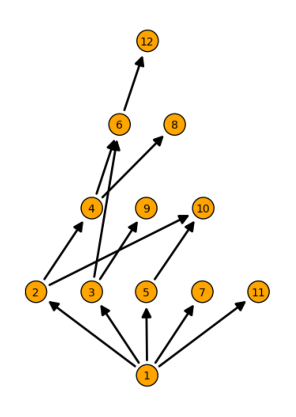
\includegraphics{Sol_9-16_gr1.eps}

\)



      (b)  The ordering diagram for \(\leq\) is a chain

\begin{doublespace}
\noindent\(\pmb{\text{                  }}\)
\end{doublespace}

</p></answer>


*************
3
*************
<answer><p> (a) \(4 \lor  8 = 8\), \(3 \lor  15 = 15\), \(4 \land  8 = 4\), \(3 \land  15 = 3\), \(3 \land  5 - 15\).



    (b)Yes. Let \(a, b, c \in P\) and assume that there are <m>n</m> primes, \(p_1\), \(p_2\), $\ldots $, \(p_n\) that appear as factors of
<m>a</m>, <m>b</m> and <m>c</m>. Then we can write



\(a = p_1{}^{i_1}p_2{}^{i_2}\cdots  p_n{}^{i_n}\)



 \(b= p_1{}^{j_1}p_2{}^{j_2}\cdots  p_n{}^{j_n}\)



\(c= p_1{}^{k_1}p_2{}^{k_2}\cdots  p_n{}^{k_n}\)



where each exponent is a nonnegative integer. The greatest common divisor and least common multiple of two integers such as <m>a</m> and \textit{
b} can be expressed in terms of these exponents.



\(a \land  b = \gcd (a, b)\text{  }= p_1{}^{m_1}p_2{}^{m_2}\cdots  p_n{}^{m_n}\) 



where \(m_r=\min \left(i_r, j_r\right)\) and



\(a \lor  b = \text{lcm}(a, b)\text{  }= p_1{}^{M_1}p_2{}^{M_2}\cdots  p_n{}^{M_n}\) 



where \(M_r=\max \left(i_r, j_r\right)\).



Based on this observation, we can compare \(a \land  (b \lor  c )\) and \(( a\land b) \lor  (a \land c)\). The exponent of p, is \(\min \left(i_r,\max
\left(j_r, k_r \right)\right)\) in \(a \land  (b \lor  c )\) and \(\max \left(\min \left(i _r , j_r\right), \min \left(i_r , k _r \right)\right)\)
in \((a \land  b) \lor  (a \land  c)\). These two exponents are equal; this is easiest to verify by checking the possible relative sizes of \(i_r\),
\(j_r\) and \(k_r\).  Therefore, the lattice is distributive.

</p></li>
<li><p> The least element is 1. There is no greatest element.

</p></answer>


*************
5
*************
<answer><p> (a) The ordering diagram is the one-cube in Figure 9.4.5. It is interesting to note that the poset relation is really the logical implication,
\(\Rightarrow\),  since \(0\Rightarrow  0\),  \(0 \Rightarrow 1\), \(1 \Rightarrow  1\) are all true statements.

</p></li>
<li><p>From the definitions of lub and glb and part (a) we have the tables



\(\begin{array}{c|c}
 \land  &amp; 
\begin{array}{cc}
 0 &amp; 1 \\
\end{array}
 \\
\hline
 
\begin{array}{c}
 0 \\
 1 \\
\end{array}
 &amp; 
\begin{array}{cc}
 0 &amp; 0 \\
 0 &amp; 1 \\
\end{array}
 \\
\end{array}\)     \(\begin{array}{c|c}
 \lor  &amp; 
\begin{array}{cc}
 0 &amp; 1 \\
\end{array}
 \\
\hline
 
\begin{array}{c}
 0 \\
 1 \\
\end{array}
 &amp; 
\begin{array}{cc}
 0 &amp; 1 \\
 1 &amp; 1 \\
\end{array}
 \\
\end{array}\)



which are the logical tables for the connectives {``}and{''} and {``}or.{''}

</p></li>
<li><p> \(L ^2 = L \times  L = \{(0, 0), (0, 1), (1, 0), (1, 1)\}\) where the poset relation $\leq $ on \(L^2\) and the binary operations $\land $ and
$\lor $ are all defined componentwise so that, for example, \((0, 1) \leq  (1, 1)\), since in the two first coordinates, \(0\leq 1\) and in the two
second coordinates, \(1\leq 1\). Also, for example, \((0, 1) \land  (1, 0) = (0 \land  1, 1 \land  0) = (0, 0)\). The operation tables are given
in the solution of Exercise 1 Section 13.5. The Hasse diagram for \(L^2\) is the two-cube.

</p></li>
<li><p> The Hasse diagram for \(L^3\) is the three-cube.  Tables for $\land $ and $\lor $ can



easily be constructed where, for example,



 \((1, 0, 0) \lor  (0, 1, 0) = (1 \lor  0,0\lor 1,0\lor 0)=(1,1,0)\)

</p></answer>


*************
7
*************
<answer><p> (a) No. It is not true that every pair of elements in <m>A</m> has both a \textit{ lub} and a \textit{ glb}



in <m>A</m>.  For example, \(10 \lor  4\) does not exist in \textit{ A.}

</p></li>
<li><p>  Yes. For all \(a, b \in  A\), \(a \neq b\),



 \(a \lor  b = \text{the} \text{maximum} \text{of} a \text{and} b\),



 \(a \land  b = \text{the} \text{minimum} \text{of} a \text{and} b.\)</p></answer>


*************
9
*************
<answer><p> \(\text{            }(x + y) \cdot  \left(x + \bar{y}\right) =x + \left(y \cdot \bar{y}\right)\text{   }\text{by} \text{the} \text{distributive}
\text{law} \text{of} + \text{over} \cdot \text{$\quad \quad $        }= x + 0\text{          }\text{by} \text{the} \text{complement} \text{law}\quad
\quad \quad = x\text{                    }\text{by} \text{the} \text{identity} \text{law}\)



The switching circuit diagram has a single switch labeled <m>x</m>.

</p></answer>


*************
11
*************
<answer><p><ol label="a">
<li><p>



\(\begin{array}{c|c}
 x &amp; \text{complement}(s) \text{of} x \\
\hline
 
\begin{array}{c}
 0 \\
 a_1 \\
 a_2 \\
 a_3 \\
 a_4 \\
 a_5 \\
 a_6 \\
 1 \\
\end{array}
 &amp; 
\begin{array}{c}
 1 \\
 a_2,a_3,a_4,a_6 \\
 a_1,a_5 \\
 a_1,a_5 \\
 a_1,a_5 \\
 a_2,a_3,a_4,a_6 \\
 a_1,a_5 \\
 0 \\
\end{array}
 \\
\end{array}\)

</p></li>
<li><p>  No, it is not distributive, for if it were, complements would be unique.</p></answer>


*************
13
*************
<answer><p> (a) \(D _{20} = \{1, 2, 4, 5, 10, 20\}\) contains 6 elements and so cannot be a Boolean algebra by Corollary 13.4.1.

</p></li>
<li><p>  \(D_{27}=\{1,3,9, 27\}\) has four elements and so we cannot use Corollary 13.4.1 to rule it out as a Boolean algebra. However, 3 has no complement,
which means that \(D_{27}\) is not a Boolean algebra.

</p></li>
<li><p>  \(D_{35} = \{1, 5, 7, 35\}\) has \(4 = 2^2\) elements, and so that it may be a Boolean algebra by Corollary 13.4.1.  We can confirm through
the definition of a Boolean algebra that it is.

</p></li>
<li><p> Notice that \(210=2\cdot 3\cdot 5\cdot 7\), which means that  \(\left\left| D_{210}\right\right|  = 16 =2^4\) and so Corollary 13.4.1 can{'}t
be used to rule it out as a Boolean algebra.  Indeed,  \(D_{210}\) is a Boolean algebra, which can be confirmed by applying the definition of
a Boolean algebra.

</p></answer>


*************
15
*************
<answer><p> (a) First, by definition of subsystem in Section 11.5, a sub-Boolean algebra of a Boolean algebra <m>B</m> is a subset <m>W</m> of \textit{
B} which is a Boolean algebra under the same operations as <m>B</m>.  Specifically, W must satisfy the conditions:

</p></li>
<li><p> The 0 and 1 of <m>B</m> must be in <m>W</m>,



(ii) \(a \in  W \Rightarrow  \bar{a} \in  W\)



(iii) \(a,b\in W\Rightarrow a\lor b\in W \text{and} a\land b\in W\). 



Hence if <m>W</m> is to contain 4 elements it must be of the form \(\left\{0, \beta , \bar{\beta }, 1\right\}\). \(W_1 = \{(0, 0, 0), (0, 1, 1),
(1, 0, 0), (1,1, 1)\}\) is one such set. The 3-cube below illustrates this sub-Boolean algebra.

\begin{doublespace}
\noindent\(\)
\end{doublespace}



 There are two others that are isomorphic to this one, where Corollary 13.4.2, assures us of this isomorphism.

</p></li>
<li><p>Again, the form of the sub-Boolean algebra with four elements must be \(\left\{0, \beta , \overline{\beta ,} 1\right\}\). Since the \(2^n\) elements
of \(B_2{}^n\) can be paired up with their complements to give us \(2^{n-1}\) pairs, there are \(2^{n-1}-1\)  ways to select the elements $\beta
$ and \(\bar{\beta }\) (0 and its complement, 1, are already selected).  Of course, all of these sub-Boolean algebras are isomorphic.

</p></li>
<li><p>A sub-Boolean algebra with \(2^k\) elements must have <m>k</m> atoms; so the selection of <m>k</m> elements that will act as atoms can be
considered in counting numbers of sub-Boolean algebras of a certain size.  What is the number?  We leave it to the reader in the general case.

</p></answer>


*************
17
*************
<answer><p>  \(\left(\overline{x_1}\land x_2\land x_3\right)\lor \left(\overline{x_1}\land \overline{x_2}\land x_3\right)\lor \left(x_1\land x_2\land x_3\right)\)

</p></answer>


*************
19
*************
<answer><p><ol label="a">
<li><p> Since each of the three variables can be any one of two values there are \(2^3\) rows, (See Table 13.6.3 for an example.) For \textit{
n} variables there are \(2^n\) rows. 

</p></li>
<li><p> For each row, there can be any one of two truth values. Since there are \(2^3=8\)  rows there are \(2^8= 256\) functions. For <m>n</m> variables
and \(m =2^n\) rows, there are \(2^m=2^{2^n}\) functions.

\begin{doublespace}
\noindent\(\)
\end{doublespace}

\begin{doublespace}
\noindent\(\)
\end{doublespace}

</p></li>
<li><p>   \(f\left(x_1,x_2,x_3\right)=\left(\left(x_1+ x_2+x_3\right)\cdot \overline{x_1}+x_1+\overline{x_2}\right)\cdot x_1\cdot \overline{x_3}\\
\\
\quad \quad =\left(x_1\cdot \overline{x_1}+ x_2\cdot \overline{x_1}+x_3\cdot \overline{x_1}+x_1+\overline{x_2}\right)\cdot x_1\cdot \overline{x_3}\\
\\
\quad \quad =\left(0+ x_2\cdot \overline{x_1}+x_3\cdot \overline{x_1}+x_1+\overline{x_2}\right)\cdot x_1\cdot \overline{x_3}\\
\\
\quad \quad =\left( x_2\cdot \overline{x_1}+x_3\cdot \overline{x_1}+x_1+\overline{x_2}\right)\cdot x_1\cdot \overline{x_3}\\
\\
\quad \quad = x_2\cdot \overline{x_1}\cdot x_1\cdot \overline{x_3}+x_3\cdot \overline{x_1}\cdot x_1\cdot \overline{x_3}+x_1\cdot x_1\cdot \overline{x_3}+\overline{x_2}\cdot
x_1\cdot \overline{x_3}\\
\\
\quad \quad = x_2\cdot 0\cdot \overline{x_3}+x_3\cdot 0\cdot \overline{x_3}+x_1\cdot \overline{x_3}+\overline{x_2}\cdot x_1\cdot \overline{x_3}\\
\\
\quad \quad =x_1\cdot \overline{x_3}+\overline{x_2}\cdot x_1\cdot \overline{x_3}\\
\\
\quad \quad =x_1\cdot \overline{x_3} \cdot \left(1+\overline{x_2}\right)\)



       Switching and gate diagrams to be added.

</p></answer>


*************
23
*************
<answer><p> (a)   \(z =\left(\overline{x_1}+x_2\right)+ \overline{x_2\cdot x_3}\)

</p></li>
<li><p>    \(z=\left(\overline{x_1}+x_2\right)+ \overline{x_2\cdot x_3}\\
\\
\quad =\left(\overline{x_1}+x_2\right)+ \left(\overline{x_2}+\overline{x_3}\right)\\
\\
\quad =\overline{x_1}+\left(x_2+ \overline{x_2}\right)+\overline{x_3}\\
\\
\quad =\overline{x_1}+1+\overline{x_3}\\
\\
\quad =1\)



     The circuit is always on, no gates are necessary.


\subsection{CHAPTER 14}


\subsubsection{Section 14.1}

*************
1.
*************
<answer><p> (a) \(S_1\) is not a submonoid since the identity of \(\left[\mathbb{Z}_8 ,\times _8\right]\), which is 1, is not in \(S_1\).   \(S_2\) is a
submonoid since \(1 \in  S_2\) and \(S_2\) is closed under multiplication; that is, for all \(a, b \in  S_2\), \(a\times _8b\) is in \(S_2\).

</p></li>
<li><p>The identity of \(\mathbb{N}^{\mathbb{N}}\) is the identity function \(i:\mathbb{N}\to \mathbb{N}\) defined by \(i(a) = a\), \(\forall a\in \mathbb{N}\).
If \(a \in \mathbb{N}\), \(i(a) = a \leq  a\), thus the identity of \(\mathbb{N}^{\mathbb{N}}\) is in \(S_1\). However, the image of 1 under any
function in \(S_2\) is 2, and thus the identity of \(\mathbb{N}^{\mathbb{N}}\) is not in \(S_2\), so \(S_2\) is not a submonoid. The composition
of any two functions in \(S_1\),  <m>f</m> and <m>g</m>, will be a function in \(S_1\):



  \(\text{        }(f\circ g)(n)= f(g(n)) \leq g(n)\text{   }\text{since} f \text{is} \text{in} S_1\quad \quad \quad \leq n\text{    }\text{since}
g \text{is} \text{in} S_1\)



Thus \(f\circ g\in S_1\), and the two conditions of a submonoid are satisfied and \(S_1\) is a submonoid of  \(\mathbb{N}^{\mathbb{N}}\) .

</p></li>
<li><p>  The first set is a submonoid, but the second is not since the null set has a non-finite complement.

</p></answer>


*************
3
*************
<answer><p> The set of \(n \times  n\) real matrices is a monoid under matrix multiplication. This follows from the laws of matrix algebra in Chapter 5. To
prove that the set of stochastic matrices is a monoid over matrix multiplication, we need only show that the identity matrix is stochastic (this
is obvious) and that the set of stochastic matrices is closed under matrix multiplication. Let <m>A</m> and <m>B</m> be \(n \times  n\) stochastic
matrices.



 \((A B)_{i j}= \sum _{k=1}^n a_{i k} b_{k j}\)



The sum of the \(j^{\text{th}}\) column is



\(\text{           }\sum _{j=1}^n (A B)_{i j}=\sum _{k=1}^n a_{1 k} b_{k j}+\sum _{k=1}^n a_{1k} b_{k j}+\cdots +\sum _{k=1}^n a_{n k} b_{k
j}\quad \quad =\sum _{k=1}^n \left(a_{1 k} b_{k j}+a_{1k} b_{k j}+\cdots +a_{n k} b_{k j}\right)\quad \quad =\sum _{k=1}^n b_{k j}\left(a_{1 k} +a_{1k}+\cdots
+a_{n k} \right)\text{  }\quad \quad = \sum _{k=1}^n  b_{k j}\text{               }\text{since} A \text{is} \text{stochastic}\quad \quad = 1\text{
                           }\text{since} B \text{is} \text{stochastic}\)


\subsubsection{Section 14.2}

*************
1.
*************
<answer><p> (a) For a character set of 350 symbols, the number of bits needed for each character is the smallest <m>n</m> such that \(2^n\) is greater
than or equal to 350.  Since   \(2^9= 512> 350 > 2^8\) ,  9 bits are needed, 

</p></li>
<li><p> \(2^{12}=4096>3500>2^{11}\); therefore, 12 bits are needed.</p></answer>


*************
3
*************
<answer><p> This grammar defines the set of all strings over <m>B</m> for which each string is a palindrome (same string if read forward or backward).


</p></answer>


*************
5
*************
<answer><p> (a) Terminal symbols: The null string, 0, and 1.



         Nonterminal symbols: \textit{ S, E.} 



         Starting symbol: S.



         Production rules: \(S\to 00S\), \(S\to 01S\),  \(S\to 10S\),  \(S\to 11S\),  \(S\to E\),  \(E\to 0\),  \(E\to 1\)



         This is a regular grammar.



    (b)Terminal symbols: The null string,  0,  and 1. 



Nonterminal symbols: <m>S</m>, <m>A</m>, <m>B</m>, <m>C</m> 



Starting symbol: <m>S</m>



Production rules: \(S \to  0A\), \(S \to  1A\), S $\to $ $\lambda $, \(A \to  0B\), \(A \to  1B\), \(A \to  \lambda\), \(B \to  0C\), \(B \to  1C\),
\(B \to  A\), \(C \to  0\), \(C \to  1\), \(C \to  \lambda\) 



 This is a regular grammar.



   </p></li>
<li><p>See Exercise 3. This language is not regular.

</p></answer>


*************
7
*************
<answer><p> If <m>s</m> is in \(A^*\) and <m>L</m> is recursive, we can answer the question {``}Is s in \(L^c\)?{''}  by



negating the answer to {``}Is <m>s</m> in <m>L</m>?$\texttt{"}$</p></answer>


*************
9
*************
<answer><p> (a) List the elements of each set \(x_i\)  in a sequence \(x_{i 1}\), \(x_{i 2}\), \(x_{i 3}\), $\ldots $ .   


\includegraphics{Sol_9-16_gr2.eps}



Then draw arrows as shown above and list the elements of the union in order established by this pattern:  \(x_{11}\), \(x_{21}\), \(x_{12}\), \(x_{13}\),
\(x_{22}\), \(x_{31}\), \(x_{41}\), \(x_{32}\), \(x_{23}\), \(x_{14}\), \(x_{15}\), $\ldots $

</p></li>
<li><p>  Each of the sets \(A^1\) , \(A^2\) , \(A^3\) , $\ldots $ are countable and \(A^*\) is the union of these sets; hence \(A^*\) is countable.


\subsubsection{Section 14.3}



  \(\begin{array}{cccc}
 x &amp; s &amp; Z(x,s) &amp; t(x,s) \\
 \text{Deposit} 25\not{c} &amp; \text{Locked} &amp; \text{Nothing} &amp; \text{Select} \\
 \text{Deposit} 25\not{c} &amp; \text{Select} &amp; \text{Return} 25\not{c} &amp; \text{Select} \\
 \text{Press} S &amp; \text{Locked} &amp; \text{Nothing} &amp; \text{Locked} \\
 \text{Press} S &amp; \text{Select} &amp; \text{Dispense} S &amp; \text{Locked} \\
 \text{Press} P &amp; \text{Locked} &amp; \text{Nothing} &amp; \text{Locked} \\
 \text{Press} P &amp; \text{Select} &amp; \text{Dispense} P &amp; \text{Locked} \\
 \text{Press} B &amp; \text{Locked} &amp; \text{Nothing} &amp; \text{Locked} \\
 \text{Press} B &amp; \text{Select} &amp; \text{Dispense} B &amp; \text{Locked} \\
\end{array}\)

\begin{doublespace}
\noindent\(\)
\end{doublespace}

</p></answer>


*************
3
*************
<answer><p>  \(\{000,011, 101, 110, 111\}\)

</p></answer>


*************
5
*************
<answer><p> (a) Input:10110, Output: 11011 \(\Rightarrow\) 10110 is in position 27 



         Input: 00100, Output: 00111 \(\Rightarrow\) 00100 is in position 7 



         Input:11111, Output: 10101 \(\Rightarrow\) 11111 is in position 21

</p></li>
<li><p>  Let \(x=x_1x_2\ldots  x_n\) and recall that for \(n\geq 1\),  \(G_{n+1}=\left(
\begin{array}{c}
 0G_n \\
 1G_n{}^r \\
\end{array}
\right)\), where \(G_n{}^r\) is the reverse of \(G_n\). To prove that the Gray Code Decoder always works, let \(p(n)\) be the proposition $\texttt{"}$Starting
in Copy state,  <m>x</m>'s output is the position of <m>x</m> in \(G_n\);  and starting in Complement state, <m>x</m>'s output is the
position of <m>x</m> in \(G_n{}^r\).$\texttt{"}$ That p(1) is true is easy to verify for both possible values of <m>x</m>,  0 and 1.  Now
assume that for some \(n\geq 1\), \(p(n)\) is true and consider \(x=x_1x_2\ldots  x_nx_{n+1}\). 



If \(x_1=0\),



    \(\text{            }x's \text{output}=0 \text{followed} \text{by} \left(x_2\ldots  x_nx_{n+1}\right)'s \text{output} \text{starting} \text{in}
\text{Copy}\text{$\quad \quad $ }=0 \text{followed} \text{by} \left(x_2\ldots  x_nx_{n+1}\right)'s \text{position} \text{in} G_n\text{$\quad \quad
$ }= x's \text{position} \text{in} G_{n+1}\) 



If  \(x_1=1\),



    \(\text{            }x's \text{output}=1 \text{followed} \text{by} \left(x_2\ldots  x_nx_{n+1}\right)'s \text{output} \text{starting} \text{in}
\text{Complement}\text{$\quad \quad $ }=1 \text{followed} \text{by} \left(x_2\ldots  x_nx_{n+1}\right)'s \text{position} \text{in} G_n{}^r\text{$\quad
\quad $ }= x's \text{position} \text{in} G_{n+1}\) 


\subsubsection{Section 14.4}

*************
1.
*************
<answer><p>   \(\begin{array}{c|c}
 \text{Input} \text{String} &amp; 
\begin{array}{cccccc}
 \text{    }a\text{       } &amp; b\text{          } &amp; \text{  }c &amp; \text{\textit{       }\text{aa}\text{         }} &amp; \text{\textit{ab}\text{      
 }} &amp; \text{\textit{ac}} \\
\end{array}
 \\
\hline
 
\begin{array}{c}
 1 \\
 2 \\
 3 \\
\end{array}
 &amp; 
\begin{array}{cccccc}
 (a,1) &amp; (a,2) &amp; (c,3) &amp; (a,1) &amp; (a,2) &amp; (c,3) \\
 (a,2) &amp; (a,1) &amp; (c,3) &amp; (a,2) &amp; (a,1) &amp; (c,3) \\
 (c,3) &amp; (c,3) &amp; (c,3) &amp; (c,3) &amp; (c,3) &amp; (c,3) \\
\end{array}
 \\
\end{array}\)



      \(\begin{array}{c|c}
 \text{Input} \text{String} &amp; \text{   }
\begin{array}{cccccc}
 \text{\textit{ba}} &amp; \text{\textit{  }\text{  }\text{     }\text{bb}\text{   }\text{  }\text{   }} &amp; \text{\textit{bc}\text{    }\text{  }\text{
  }} &amp; \text{\textit{ca}\text{          }} &amp; \text{\textit{cb}\text{    }} &amp; \text{\textit{cc}\text{      }} \\
\end{array}
 \\
\hline
 
\begin{array}{c}
 1 \\
 2 \\
 3 \\
\end{array}
 &amp; 
\begin{array}{cccccc}
 (a,2) &amp; (a,1) &amp; (c,3) &amp; (c,3) &amp; (c,3) &amp; (c,3) \\
 (a,1) &amp; (a,2) &amp; (c,3) &amp; (c,3) &amp; (c,3) &amp; (c,3) \\
 (c,3) &amp; (c,3) &amp; (c,3) &amp; (c,3) &amp; (c,3) &amp; (c,3) \\
\end{array}
 \\
\end{array}\)



We can see that \(T_aT_a= T_{\text{\textit{aa}}}=T_a\),  \(T_aT_b= T_{\text{\textit{ab}}}= T_b\), etc. Therefore, we have the following monoid:



          \(\begin{array}{c|c}
   &amp; 
\begin{array}{ccc}
 \text{   }T_{a\text } &amp; T_b &amp;  T_b \\
\end{array}
 \\
\hline
 
\begin{array}{c}
 T_a \\
 T_b \\
 T_c \\
\end{array}
 &amp; 
\begin{array}{ccc}
 T_a &amp; T_b &amp; T_c \\
 T_b &amp; T_a &amp; T_c \\
 T_c &amp; T_c &amp; T_c \\
\end{array}
 \\
\end{array}\)



Notice that \(T_a\) is the identity of this monoid.

</p></li>
<li><p>   \(\begin{array}{c|c}
 \text{Input} \text{String} &amp; 
\begin{array}{cccccc}
 \text{   }1 &amp; \text{  }2  &amp;  11 &amp; 12 &amp; 21 &amp; 22 \\
\end{array}
 \\
\hline
 
\begin{array}{c}
 A \\
 B \\
 C \\
 D \\
\end{array}
 &amp; 
\begin{array}{cccccc}
 C &amp; B &amp; A &amp; D &amp; D &amp; A \\
 D &amp; A &amp; B &amp; C &amp; C &amp; B\text{} \\
 A\text{} &amp; D\text{} &amp; C\text{} &amp; B &amp; B &amp; C \\
 B &amp; C &amp; D &amp; A &amp; A &amp; D \\
\end{array}
 \\
\end{array}\)



        \(\begin{array}{c|c}
 \text{Input} \text{String} &amp; 
\begin{array}{cccccccc}
 \text{   }111 &amp; 112 &amp; 121 &amp; 122 &amp; 211\text{\textit{$ $}} &amp; 212 &amp; 221 &amp; 222 \\
\end{array}
 \\
\hline
 
\begin{array}{c}
 A \\
 B \\
 C \\
 D \\
\end{array}
 &amp; 
\begin{array}{cccccccc}
 C\text{     } &amp; B\text{     } &amp; B\text{     } &amp; C\text{     } &amp; B\text{     } &amp; C\text{     } &amp; C\text{    } &amp; B \\
 D\text{    } &amp; A\text{    } &amp; A\text{     } &amp;  D\text{    } &amp; A\text{    } &amp; D\text{     } &amp; D\text{   } &amp; A \\
 B\text{    } &amp; C\text{    } &amp; C\text{    } &amp; B\text{   } &amp; C\text{    } &amp; B\text{    } &amp; B\text{   } &amp; C \\
 B\text{    } &amp; C\text{    } &amp; C\text{    } &amp; B\text{   } &amp; C\text{    } &amp; B\text{    } &amp; B\text{   } &amp; C \\
\end{array}
 \\
\end{array}\)



We have the following monoid:



          \(\begin{array}{c|c}
   &amp; 
\begin{array}{cccc}
 T_1 &amp;  T_2 &amp; \text{  }T_{11} &amp;  T_{12} \\
\end{array}
 \\
\hline
 
\begin{array}{c}
 T_1 \\
 T_2 \\
 T_{11} \\
 T_{12} \\
\end{array}
 &amp; 
\begin{array}{cccc}
 T_{11} &amp; T_{12} &amp; T_1 &amp; T_2 \\
 T_b &amp; T_{11} &amp; T_2 &amp; T_1 \\
 T_1 &amp; T_2 &amp; T_{11} &amp; T_{12} \\
 T_2 &amp; T_1 &amp; T_{12} &amp; T_{11} \\
\end{array}
 \\
\end{array}\)



Notice that \(T_{11}\) is the identity of this monoid.

</p></answer>


*************
3
*************
<answer><p> Yes, just consider the unit time delay machine of Figure 14.4.2. Its monoid is described by the table at the end of Section 14.4 where the \(T_{\lambda
}\) row and \(T_{\lambda }\) column are omitted. Next consider the machine in Figure 14.5.3. The monoid of this machine is:



     \(\begin{array}{c|ccccccc}
   &amp; T_{\lambda } &amp; T_0 &amp; T_1 &amp; T_{00} &amp; T_{01} &amp; T_{10} &amp; T_{11} \\
\hline
 T_{\lambda } &amp; T_{\lambda } &amp; T_0 &amp; T_1 &amp; T_{00} &amp; T_{01} &amp; T_{10} &amp; T_{11} \\
\hline
 T_0 &amp; T_0 &amp; T_{00} &amp; T_{01} &amp; T_{00} &amp; T_{01} &amp; T_{10} &amp; T_{11} \\
 T_1 &amp; T_1 &amp; T_{10} &amp; T_{11} &amp; T_{00} &amp; T_{01} &amp; T_{10} &amp; T_{11} \\
 T_{00} &amp; T_{00} &amp; T_{00} &amp; T_{01} &amp; T_{00} &amp; T_{01} &amp; T_{10} &amp; T_{11} \\
 T_{01} &amp; T_{01} &amp; T_{10} &amp; T_{11} &amp; T_{00} &amp; T_{01} &amp; T_{10} &amp; T_{11} \\
 T_{10} &amp; T_{10} &amp; T_{00} &amp; T_{01} &amp; T_{00} &amp; T_{01} &amp; T_{10} &amp; T_{11} \\
 T_{11} &amp; T_{11} &amp; T_{10} &amp; T_{11} &amp; T_{00} &amp; T_{01} &amp; T_{10} &amp; T_{11} \\
\end{array}\)



Hence both of these machines have the same monoid, however, their transition diagrams are nonisomorphic since the first has two vertices and the
second has seven.


\subsubsection{Section 14.5}

*************
1.
*************
<answer><p> </p></li>
<li><p>

\begin{doublespace}
\noindent\(\pmb{}\)
\end{doublespace}



 (b)

\begin{doublespace}
\noindent\(\pmb{}\)
\end{doublespace}


\subsubsection{Supplementary Exercises$---$Chapter 14}

*************
1.
*************
<answer><p>   Let \(f, g, h \in  M\), and \(a \in  B\).



\(((f*g)*h)(a) = (f*g)(a) \land  h(a)\\
\\
\quad \quad = (f(a)\land g(a))\land h(a)\\
\\
\quad \quad = f(a) \land ( g(a) \land  h(a))\\
\\
\quad \quad = f(a) \land  (g * h)(a)\\
\\
\quad \quad = (f * (g * h))(a)\)



Therefore \((f * g) * h =f * (g * h) \Rightarrow  * \text{is} \text{associative}\).



The identity for \(*\) is the function \(u \in  M\) where \(u (a) = 1\) = the {``}one{''} of <m>B</m>. If \(a \in  B\)



\((f*u)(a) =f(a)\land u(a) = f(a)\land 1 = f(a)\)



Therefore \(f * u - f\). Similarly\(u * f =f\).



There are \(2^2= 4\) functions in \(M\) for \(B = B _2\). These four functions are named in the text (see Figure 14.1.1). The table for \(*\) is



          \(\begin{array}{c|c}
   &amp; 
\begin{array}{cccc}
 z &amp;  i &amp; \text{  }t &amp;  u \\
\end{array}
 \\
\hline
 
\begin{array}{c}
 z \\
 i \\
 t \\
 u \\
\end{array}
 &amp; 
\begin{array}{cccc}
 z &amp; z &amp; z &amp; z \\
 z &amp; i &amp; z &amp; i \\
 z &amp; z &amp; t &amp; t \\
 z &amp; u &amp; t &amp; u \\
\end{array}
 \\
\end{array}\)

</p></answer>


*************
3
*************
<answer><p>   \(\{a,\text{\textit{$ $}}\text{\textit{bb}, \text{bbb}, \text{bbbb}}, . . .\}\)

</p></answer>


*************
5
*************
<answer><p>    S = start symbol. Nonterminals = \(\left\{S, B_0 , B_1, B_2\right\}\)



\(\text{          }S\to B_0\text{        }B_0\text{-$>$}a B_0\text{    }B_0\to b B_1\quad \quad B_1\to a B_1\text{       }B_1\to b B_2\text{
     }B_1\to b\quad \quad B_2 \to a B_2\text{      }B_2\to a\)

</p></answer>


*************
7
*************
<answer><p> 

\begin{doublespace}
\noindent\(\)
\end{doublespace}

</p></answer>


*************
9
*************
<answer><p> </p></li>
<li><p>

\begin{doublespace}
\noindent\(\pmb{}\)
\end{doublespace}

</p></li>
<li><p> The possible output sequences are 100, 010, 001, and 111. Note: Output for \(t = 3\) is determined by the next state, \(s(4)\)). If \(s(4) =
s(3)\), output at \(t = 3\) is 0, while if \(s(4) \neq  s(3)\), output at \(t=3\) is 1.</p></answer>


*************
11
*************
<answer><p>

\begin{doublespace}
\noindent\(\)
\end{doublespace}


\section{CHAPTER 15}


\subsection{Section 15.1}

*************
1.
*************
<answer><p>  The only other generator is \(-1\).

</p></answer>


*************
3
*************
<answer><p>  If  \(\left| G\right| =m\)  , \(m>2\), and \(G = \langle a\rangle\), then <m>a</m>, \(a^2,\ldots\), \(a^{m-1}\) , \(a^m=e\) are distinct
elements of <m>G</m>. Furthermore, \(a^{-1}= a^{m-1}\neq a\),  If \(1\leq k\leq m\),  \(a^{-1}\) generates \(a^k\):



   \(\text{               }\left(a^{-1}\right)^{m-k}= \left(a^{m-1}\right)^{m-k}= a^{m^2-m-m k + k}\quad \quad =\left(a^m\right)^{m-k-1}*a^k=
e*a^k=a^k\)



Similarly, if <m>G</m> is infinite and \(G = \langle a\rangle\), then \(a^{-1}\) generates <m>G</m>.</p></answer>


*************
5
*************
<answer><p> (a) No. Assume that \(q \in \mathbb{Q}\) generates $\mathbb{Q}$. Then \(\langle q\rangle  = \{n q : n \in \mathbb{Z}\}\). But this gives us at
most integer multiples of <m>q</m>, not every element in $\mathbb{Q}$.

</p></li>
<li><p> No. Similar reasoning to part a.

</p></li>
<li><p> Yes. 6 is a generator of \(6\mathbb{Z}\).

</p></li>
<li><p>  No.

</p></li>
<li><p> Yes, \((1,1, 1)\) is a generator of the group.

</p></answer>


*************
7
*************
<answer><p> Theorem 15.1.4 implies that <m>a</m> generates \(\mathbb{Z}_n\) if and only if the greatest common divisor of <m>n</m> and <m>a</m> is
1 (i. e., <m>n</m> and <m>a</m> are relatively prime). Therefore the list of generators of \(\mathbb{Z}_n\) are the integers in \(\mathbb{Z}_n\)
that are relatively prime to <m>n</m>. The generators of \(\mathbb{Z}_{25}\) are all of the nonzero elements except 5, 10, 15, and 20. The generators
of \(\mathbb{Z}_{256}\) are the odd integers in \(\mathbb{Z}_{256}\)  since 256 is \(2^8\).  \textit{ Mathematica} expression to generate these
sets are

\begin{doublespace}
\noindent\(\pmb{\text{Select}[\text{Range}[0,24],\text{Function}[a,\text{GCD}[25,a]==1]]}\)
\end{doublespace}

\begin{doublespace}
\noindent\(\{1,2,3,4,6,7,8,9,11,12,13,14,16,17,18,19,21,22,23,24\}\)
\end{doublespace}

\begin{doublespace}
\noindent\(\pmb{\text{Select}[\text{Range}[0,255],\text{Function}[a,\text{GCD}[256,a]==1]]}\)
\end{doublespace}

\begin{doublespace}
\noindent\(\{1,3,5,7,9,11,13,15,17,19,21,23,25,27,29,31,33,35,37,39,41,43,45,47,49,51,53,55,57,59,61,63,65,67,69,71,73,75,77,79,81,83,85,87,89,91,93,95,97,99,101,103,105,107,109,111,113,115,117,119,121,123,125,127,129,131,133,135,137,139,141,143,145,147,149,151,153,155,157,159,161,163,165,167,169,171,173,175,177,179,181,183,185,187,189,191,193,195,197,199,201,203,205,207,209,211,213,215,217,219,221,223,225,227,229,231,233,235,237,239,241,243,245,247,249,251,253,255\}\)
\end{doublespace}

</p></answer>


*************
9
*************
<answer><p> (a)  \(\theta :\mathbb{Z}_{77} \to  \mathbb{Z}_7 \times  \mathbb{Z}_{11}\)



  \(\begin{array}{ccc}
 21 &amp; \to  &amp; (0,10) \\
 5 &amp; \to  &amp; (5,5) \\
 7 &amp; \to  &amp; (0,7) \\
 15 &amp; \to  &amp; \underline{(1,4)} \\
 \text{sum}=48 &amp; \leftarrow  &amp; (6,4)=\text{sum} \\
\end{array}\)



The final sum, 48, is obtained by using the facts that \(\theta ^{-1}(1,0) =22\) and \(\theta ^{-1}(0,1)=56\)



\(\theta ^{-1}(6,4)=6 \times _{77}\theta ^{-1}(1,0)\text{  }+ 4 \times _{77}\theta ^{-1}(0,1)\\
\\
\quad \quad =6\times _{77}22 +_{77}4\times _{77}56\\
\\
\quad \quad =55 +_{77}70\\
\\
\quad \quad =48\)

</p></li>
<li><p>  Using the same isomorphism:



\(\begin{array}{ccc}
 25 &amp; \to  &amp; (4,3) \\
 26 &amp; \to  &amp; (5,4) \\
 40 &amp; \to  &amp; (5,7) \\
   &amp;   &amp; \text{sum}=(0,3)\text{            } \\
\end{array}\)



\(\text{              }\theta ^{-1}(0,3)= 3\times _{77}\theta ^{-1}(0,1)\quad \quad = 3\times _{77}56\quad \quad =14\)



The actual sum is 91. Our result is incorrect, since 91 is not in \(\mathbb{Z}_{77}\).  Notice that 91 and 14 differ by 77. Any error that we get
using this technique will be a multiple of 77.


\subsection{Section 15.2}

*************
1.
*************
<answer><p> Call the subsets <m>A</m> and <m>B</m> respectively. If we choose \(0 \in A\) and \(\text{5 $\in $ }\text{\textit{$B$}}\) we get \(0 +_{10}
5 =5\in  B\). On the other hand, if we choose \(3 \in A\) and \(8 \in  B\), we get \(3 +_{10}8 = 1 \in  A\). Therefore, the induced operation is
not well defined on \(\{A,B\}\).

</p></answer>


*************
3
*************
<answer><p> (a) The four distinct cosets in \(G/H\) are



\(\text{                 }H = \{(0, 0), (2, 0)\}\)



  \((1, 0) + H= \{(1,0),(3,0)\}\)



 \((0, 1) + H= \{(0,1),(2,1)\}\), 



     and \((1, 1) +H= \{(1,1),(3,1)\}\) 



None of these cosets generates \(G/H\); therefore \(G/H\) is not cyclic. Hence \(G/H\) must be isomorphic to \(\mathbb{Z}_2\times \mathbb{Z}_2\)
.

</p></li>
<li><p> The factor group is isomorphic to \([\mathbb{R}; +]\). Each coset of $\mathbb{R}$ is a line in the complex plane that is parallel to the x-axis:
\(\tau :\mathbb{C}/\mathbb{R}\to  \mathbb{R}\), where \(T(\{a + b i|a\in \mathbb{R}\}) = b\) is an isomorphism.

</p></li>
<li><p>    \(\langle 8\rangle  = \{0, 4, 8, 12, 16\}\text{  }\)\(\Rightarrow\)  \(\left\left| \left.\mathbb{Z}_{20}\right/\langle 8\rangle \right\right|
=4\) .



The four cosets are: \(\bar{0}\), \(\bar{1}\), \(\bar{2}\), and \(\bar{3}\). 1 generates all four cosets.  The factor group is isomorphic to \(\left[\mathbb{Z}_4,
+_4\right]\)  because \(\bar{1}\) generates it.

</p></answer>


*************
5
*************
<answer><p> \(\text{                        }a \in b H \Leftrightarrow  a = b * h\text{    }\text{for} \text{some}h \in H\text{$\quad \quad $        }\Leftrightarrow
b^{-1}*a = h\text{  }\text{for} \text{some}h \in H\quad \quad \Leftrightarrow  b^{-1}*a \in  H\)


\subsection{Section 15.3}

*************
1.
*************
<answer><p> </p></li>
<li><p>   \(\left(
\begin{array}{cccc}
 1 &amp; 2 &amp; 3 &amp; 4 \\
 1 &amp; 4 &amp; 3 &amp; 2 \\
\end{array}
\right)\)       </p></li>
<li><p>     \(\left(
\begin{array}{cccc}
 1 &amp; 2 &amp; 3 &amp; 4 \\
 4 &amp; 3 &amp; 1 &amp; 2 \\
\end{array}
\right)\)

</p></li>
<li><p>      \(\left(
\begin{array}{cccc}
 1 &amp; 2 &amp; 3 &amp; 4 \\
 3 &amp; 4 &amp; 2 &amp; 1 \\
\end{array}
\right)\)      (d)     \(\left(
\begin{array}{cccc}
 1 &amp; 2 &amp; 3 &amp; 4 \\
 3 &amp; 4 &amp; 2 &amp; 1 \\
\end{array}
\right)\)

</p></li>
<li><p>      \(\left(
\begin{array}{cccc}
 1 &amp; 2 &amp; 3 &amp; 4 \\
 4 &amp; 2 &amp; 1 &amp; 3 \\
\end{array}
\right)\)      (f)     \(\left(
\begin{array}{cccc}
 1 &amp; 2 &amp; 3 &amp; 4 \\
 3 &amp; 1 &amp; 4 &amp; 2 \\
\end{array}
\right)\)

</p></li>
<li><p>      \(\left(
\begin{array}{cccc}
 1 &amp; 2 &amp; 3 &amp; 4 \\
 2 &amp; 1 &amp; 4 &amp; 3 \\
\end{array}
\right)\)    </p></answer>


*************
3
*************
<answer><p>  Yes and no, respectively

</p></answer>


*************
5
*************
<answer><p> \(D_4 = \left\{i, r, r^2 , r^3 , f_1 f_2,f_3, f_4\right\}\)



Where <m>i</m> is the identity function, \(r=\left(
\begin{array}{cccc}
 1 &amp; 2 &amp; 3 &amp; 4 \\
 2 &amp; 3 &amp; 4 &amp; 1 \\
\end{array}
\right)\), and 



\(\begin{array}{cc}
 f_1 =\left(
\begin{array}{cccc}
 1 &amp; 2 &amp; 3 &amp; 4 \\
 4 &amp; 3 &amp; 2 &amp; 1 \\
\end{array}
\right) &amp; f_2 =\left(
\begin{array}{cccc}
 1 &amp; 2 &amp; 3 &amp; 4 \\
 2 &amp; 1 &amp; 4 &amp; 3 \\
\end{array}
\right) \\
 f_3 =\left(
\begin{array}{cccc}
 1 &amp; 2 &amp; 3 &amp; 4 \\
 3 &amp; 2 &amp; 1 &amp; 4 \\
\end{array}
\right) &amp; f_4 =\left(
\begin{array}{cccc}
 1 &amp; 2 &amp; 3 &amp; 4 \\
 1 &amp; 4 &amp; 3 &amp; 2 \\
\end{array}
\right) \\
\end{array}\)



The operation table for the group is



\(\begin{array}{c|c}
 \circ  &amp; \text{   }
\begin{array}{cccccccc}
 i  &amp; r  &amp; r^2 &amp; r^3  &amp; f_1 &amp;  f_2\text{  } &amp; f_3 &amp; f_4 \\
\end{array}
 \\
\hline
 
\begin{array}{c}
 i \\
 r \\
 r^2 \\
 r^3 \\
 f_1 \\
 f_2 \\
 f_3 \\
 f_4 \\
\end{array}
 &amp; 
\begin{array}{cccccccc}
 i &amp; r &amp; r^2 &amp; r^3 &amp; f_1 &amp; f_2 &amp; f_3 &amp; f_4 \\
 r &amp; r^2 &amp; r^3 &amp; i &amp; f_4 &amp; f_3 &amp; f_1 &amp; f_2 \\
 r^2 &amp; r^3 &amp; i &amp; r &amp; f_2 &amp; f_1 &amp; f_4 &amp; f_3 \\
 r^3 &amp; i &amp; r &amp; r^2 &amp; f_3 &amp; f_4 &amp; f_2 &amp; f_1 \\
 f_1 &amp; f_3 &amp; f_2 &amp; f_4 &amp; i &amp; r^2 &amp; \square  &amp; r^3 \\
 f_2 &amp; f_4 &amp; f_1 &amp; f_3 &amp; r^2 &amp; i &amp; r^3 &amp; r \\
 f_3 &amp; f_2 &amp; f_4 &amp; f_1 &amp; r^3 &amp; r &amp; i &amp; r^2 \\
 f_4 &amp; f_1 &amp; f_3 &amp; f_2 &amp; r &amp; r^3 &amp; r^2 &amp; i \\
\end{array}
 \\
\end{array}\)



A lattice diagram of its subgroups is

\begin{doublespace}
\noindent\(\pmb{}\)
\end{doublespace}



All proper subgroups are cyclic except \(\left\{i,r^2,f_1,f_2\right\}\)\(\text{}\text{}\)and \(\left\{i,r^2,f_3,f_4\right\}\).  Each 2-element
subgroup is isomorphic to \(\mathbb{Z}_2\) ; \(\left\{i,r,r^2,r^3\right\}\) is isomorphic to \(\mathbb{Z}_4\) ; and \(\left\{i,r^2,f_1,f_2\right\}\)\(\text{}\text{}\)and
\(\left\{i,r^2,f_3,f_4\right\}\) are isomorphic to \(\mathbb{Z}_2\times \mathbb{Z}_2\).

</p></answer>


*************
7
*************
<answer><p>  One solution is to cite Exercise 3 at the end of Section 11.3. It can be directly applied to this problem. An induction proof of the problem
at hand would be almost identical to the proof of the more general statement.



  \(\left(t_1t_2\cdots  t_r\right){}^{-1}= t_r{}^{-1}\cdots  t_2{}^{-1}t_1{}^{-1}\text{       }\text{by} \text{Exercies} 3 \text{of} \text{Section}
11.3\\
\\
\quad \quad = t_r\cdots  t_2t_1\text{               }\text{since} \text{each} \text{transposition} \text{inverts} \text{itself}.\text{    }\blacksquare
\text{  }\)

</p></answer>


*************
9
*************
<answer><p> Part I: That \(\left\left| S_k\right\right|  = k!\) follows from Exercise 3 of Section 7.3.



Part II: Let  <m>f</m>  be the function defined on \(\{1,2,\text{...}, n\}\) by \(f(1)=2\), \(f(2)=3\),  \(f(3)=1\), and \(f(j) =j\)  for
\(4\leq j\leq n\); and let <m>g</m> be defined by \(g(1) = 1\), \(g(2) = 3\), \(g(3) = 2\), and \(g(j) =j\)  for \(4\leq j\leq n\).  Note
that <m>f</m> and <m>g</m> are elements of \(S_n\). Next, \((f\circ g)(1) = f(g(1)) = f(1) = 2\), while \((g \circ f)(1) = g(f(1)) = g(2) =
3\), hence  \(f\circ g\neq g\circ f\) and \(S_n\) is non-abelian for any \(n \geq  3\).

</p></answer>


*************
11
*************
<answer><p> (a) Both groups are non-abelian and of order 6; so they must be isomorphic, since only one such group exists up to isomorphism. The function
\(\theta :S_3\to R_3\) defined by



\(\begin{array}{cc}
 \theta (i)=I &amp; \theta \left(f_1\right)=F_1 \\
 \theta \left(r_1\right)=R_1 &amp; \theta \left(f_2\right)=F_2 \\
 \theta \left(r_2\right)=R_2 &amp; \theta \left(f_3\right)=F_3 \\
\end{array}\)



is an isomorphism,

</p></li>
<li><p> Recall that since every function is a relation, it is natural to translate functions to Boolean matrices. Suppose that \(f\in S_n\). We will
define its image, \(\theta (f)\), by 



\(\theta (f)_{\text{\textit{kj}}}=1\text{   }\Leftrightarrow \text{     }f(j)=k\)



That $\theta $ is a bijection follows from the existence of \(\theta ^{-1}\).   If <m>A</m> is a rook matrix, 



\(\text{  }\theta ^{-1}(A)(j)=k\text{  }\Leftrightarrow \text{   }\text{The} 1 \text{in} \text{column} j \text{of} A \text{appears} \text{in}
\text{row} k \quad \quad \Leftrightarrow \text{  }\text{\textit{$A_{\text{kj}}$}}=1\) 



For \(f,g\in  S_n\), 



   \(\theta (f\circ g)_{k j}= 1\text{  }\Leftrightarrow \text{   }(f \circ g)(j)=k\\
\\
\quad \quad \Leftrightarrow \text{  }\exists  l\text{  }\text{such} \text{that}\text{  }g(j)=l\text{  }\text{and} f(l)=k\\
\\
\quad \quad \Leftrightarrow \text{  }\exists  l\text{  }\text{such} \text{that}\text{  }\theta (g)_{\text{\textit{lj}}}=1\text{   }\text{and}\text{
 }\theta (f)_{k l}=1\\
\\
\quad \quad \Leftrightarrow \text{  }(\theta (f)\theta (g))_{k j}=1\)



Therefore,  $\theta $ is an isomorphism. \(\blacksquare\)


\subsection{Section 15.4}

*************
1.
*************
<answer><p> (a)  Yes, the kernel is\(\{1, -1\}\)

</p></li>
<li><p> No, since \(\theta _2\left(2 +_54\right)= \theta _2(1)=1\), but  \(\theta _2(2)+_2\theta _2(4)=0+_20 =0\)

</p></li>
<li><p> Yes, the kernel is \(\{(a, -a)| a \in \mathbb{R}\}\)

</p></li>
<li><p>  No

</p></answer>


*************
3
*************
<answer><p>  \(\langle r\rangle =\left\{i,r,r^2,r^3\right\}\) is a normal subgroup of \(D_4\). To see you could use the table given in the solution of Exercise
5 of Section 15.3 and verify that  \(a^{-1}h a \in \langle r\rangle\) for all \(a\in D_4\) and \(h\in \langle r\rangle\).   A more efficient
approach is to prove the general theorem that if <m>H</m> is a subgroup <m>G</m> with exactly two distinct left cosets, than <m>H</m> is
normal.  



\(\left\langle f_1\right\rangle\) is not a normal subgroup of \(D_4\).  \(\left\langle f_1\right\rangle =\left\{i,f_1\right\}\) and if we choose
\(a = r\) and \(h=f_1\) then \(a^{-1}h a= r^3f_1r=f_2\notin \left\langle f_1\right\rangle\)</p></answer>


*************
5
*************
<answer><p>  \((\beta \circ  \alpha )\left(a_1,a_2,a_3\right) = 0\)  and so \(\beta \circ \alpha\)  is the trivial homomorphism, but a homomorphism
nevertheless.

</p></answer>


*************
7
*************
<answer><p> Let \(x, y \in G\).



\(\text{               }q(x * y) = (x * y)^2\quad \quad = x*y *x*y\quad \quad =x * x*y *y\text{   }\text{since} G \text{is} \text{abelian}\quad
\quad =x^2*y^2\quad \quad = q(x)*q(y)\)



Hence, <m>q</m> is a homomorphism.



In order for \textit{ q }to be an isomorphism, it must be the case that no element other than the identity is its own inverse.



              \(\text{        }x \in \text{Ker} (q) \Leftrightarrow  q (x) = e \quad \quad \Leftrightarrow  x * x =e \quad \quad \Leftrightarrow
\text{  }x^{-1}= x\)

</p></answer>


*************
9
*************
<answer><p> Proof: Recall: The inverse image of \(H'\) under $\theta $ is



\(\theta ^{-1}(H')=\{g\in G | \theta (g)\in H'\}\)



Closure:   Let \(g_1g_2\in \theta ^{-1}(H')\), then \(\theta \left(g_1\right),\theta \left(g_2\right)\in H'\).  Since \(H'\) is a subgroup



of \(G'\), 



\(\theta \left(g_1\right)\diamond \theta \left(g_2\right)=\theta \left(g_1*g_2\right) \Rightarrow \text{  }g_1*g_2\in \theta ^{-1}(H')\)







Identity: By Theorem 15.4.2(a), \(e \in \theta ^{-1}(H')\).



Inverse: Let \(a\in \theta ^{-1}(H')\) . Then \(\theta (a)\in H'\) and by Theorem 15.4.2(b), \(\theta (a)^{-1}= \theta \left(a^{-1}\right)\in H'\)
and so \(a^{-1}\in \theta ^{-1}(H')\).


\subsection{Section 15.5}

*************
1.
*************
<answer><p> (a) Error detected, since an odd number of Is was received; ask for retransmission.

</p></li>
<li><p> No error detected; accept this block.

</p></li>
<li><p> No error detected; accept this block.

</p></answer>


*************
3
*************
<answer><p> (a) Syndrome = \((1, 0, 1)\). Corrected message = \((1, 1, 0)\).

</p></li>
<li><p> Syndrome =\((1, 1,0)\). Corrected message =\((0, 0, 1)\).

</p></li>
<li><p> Syndrome \((0,0,0)\). \(\text{Corrected} \text{message} =\text{received} \text{message}\\
\\
\text{$\quad \quad $        }=\text{   }(0, 1, 1)\).

</p></li>
<li><p> Syndrome = \((1, 1,0)\). Corrected message =\((1, 0, 0)\).

</p></li>
<li><p> Syndrome = \((1, 1, 1)\). This syndrome occurs only if two bits have been switched. No reliable correction is possible.

</p></answer>


*************
5
*************
<answer><p> Let <m>G</m> be the \(9\times 10\) matrix obtained by augmenting the \(9\times 9\) identity matrix with a column of ones. The function \(e
:\mathbb{Z}_2{}^9\to \mathbb{Z}_2{}^{10}\)  defined by \(e(a) = a G\) will allow us to detect single errors, since \(e(a)\) will always have an
even number of ones.


\subsection{Supplementary Exercises$---$Chapter 15}

*************
1.
*************
<answer><p> Theorem 15.1.3 guarantees that all subgroups of any cyclic group can be determined by finding all cyclic subgroups. We can find all cyclic subgroups
of noncyclic groups but there may be other subgroups.</p></answer>


*************
3
*************
<answer><p> First, write 120 as a product of powers of distinct primes: \(120 = 2^3\cdot 3\cdot 5\). The Chinese Remainder Theorem states that  \(\theta
:\mathbb{Z}_{120}\to \mathbb{Z}_8\times \mathbb{Z}_3\times \mathbb{Z}_5\) defined by \(\theta (k)=((k \bmod 8), (k \bmod 3), (k \bmod 5))\)  is
an isomorphism.  In particular, \(\theta (74)=(2,2,4)\)  and \(\theta (85)=(5,1,0)\).   Therefore,



\(\theta \left(74+_{120}85\right)=\theta (74)+\theta (85)\\
\\
\quad \quad = (2,2,4)+(5,1,0)\\
\\
\quad \quad =(7,0,4)\)



Since \(\theta (105) = (1,0, 0)\), and \(\theta (96) = (0, 0, 1)\), we can compute



 $\quad \quad \quad $\(\text{      }\theta ^{-1}(7, 0, 4) = 7 \times _{120} 105\text{  }+_{120} 4 \times _{120} 96 \quad \quad = 39\).



 5.  \(H= 0 + H = \{0, 4, 8\} =4 +H = 8+H\)



\(1+H = \{1,5, 9\} = 5 + H = 9 + H\)



\(2+ H = \{2, 6, 10\} = 6 + H = 10 + H\)



\(3+ H = \{3, 7, 11\} = 7 + H = 11 + H\)



The operation table for this factor group is the same as that of \(\left[\mathbb{Z}_4,+_4\right]\) with <m>k</m> replaced with \(k+ H\).

</p></answer>


*************
7
*************
<answer><p> (a) \(\left\left| \mathbb{Z}_8\right\right|  = 8\) and \(\left| \langle 2\rangle \right| = 4\), therefore there are 2 distinct left cosets, and
they are:



\(0+ \langle 2\rangle  = \{0, 2, 4, 6\} = 2 + \langle 2\rangle  = 4 + \langle 2\rangle  = 6 + \langle 2\rangle\)



\(1+ \langle 2\rangle  = \{1, 3, 5, 7\} = 3 + \langle 2\rangle  = 5 + \langle 2\rangle  = 7 + \langle 2\rangle\)

</p></li>
<li><p>  \(\left\left| \mathbb{Z}_{12}\right\right|  = 12\) and \(\left| \langle 2\rangle \right|  = 6\), therefore there are 2 distinct left cosets
and they are:



\(0+ \langle 2\rangle  = \{(), 2, 4, 6, 8, 10\} = 2 + \langle 2\rangle  = 4 + \langle 2\rangle  - 6 + \langle 2\rangle = 8 + \langle 2\rangle
 = 10 + \langle 2\rangle\)



      and \(1+ \langle 2\rangle  = \{1, 3, 5, 7, 9, 11\} = 3 + \langle 2\rangle  = 5 + \langle 2\rangle  = 7 + \langle 2\rangle = 9 + \langle
2\rangle  = 11 + \langle 2\rangle\)

</p></li>
<li><p>  Since both groups are of order 2 and there is only one group of order 2 up to isomorphism, they are isomorphic. A simpler group is \(\mathbb{Z}_2\).

</p></answer>


*************
7
*************
<answer><p>  Assume  <m>f</m> is even,  \(f=t_1\circ t_2\circ \cdots \circ t_{2r}\)  for some \(r\), where each \(t_i\) is a transposition. Hence



\(f^{-1}=\left(t_1\circ t_2\circ \cdots \circ t_{2r}\right){}^{-1} = t_{2r}\circ \cdots \circ t_2\circ t_1\) by Exercise 11 of Section 15.3.




Since the alternative, that <m>f</m> is odd, leads to \(f^{-1}\) being odd,  \textit{ f }is even if and only if \(f^{-1}\) is even.\\
\\
11. (a) \textit{ This following is the {``}standard definition{''} of a Boolean algebra homomorphism}.  



 \(f:B_1\to B_2\) is a Boolean algebra homomorphism if and only if for all \(a, b, \in B_1\).



(1)  \(f(a\land b)=f(a)\land f(b)\)



(2)  \(f(a\lor b)=f(a)\lor f(b)\) 



(3)   \(f\left(\bar{a}\right) =\overline{ f(a)}\)

</p></li>
<li><p> (i) \(f(0) = f\left(a \land  \bar{a}\right) \\
\\
\quad = f(a) \land f\left(\overset{\text{}_{\_}}{a}\right) \\
\\
\quad = f(a) \land  \overline{f(a)} \\
\\
\quad = 0\)



and



 \(f(1) = f\left(a \lor  \bar{a}\right) \\
\\
\quad = f(a) \lor f\left(\overset{\text{}_{\_}}{a}\right) \\
\\
\quad = f(a) \lor  \overline{f(a)} \\
\\
\quad = 1\)



      Note : The 0 and 1 of \(B_1\) may be different than those of \(B_2\). 



(ii)  \(a\leq b\Rightarrow  a=a\land b\text{    }\text{by} \text{Supplementary} \text{Exercise} 4 \text{of} \text{Chapter} 13\\
\\
\quad \Rightarrow  f(a)=f(a\land b)=f(a)\land f(b)\\
\\
\quad \Rightarrow \text{  }f(a)\leq f(b)\text{   }\text{by} \text{the} \text{same} \text{exercise} \text{cited} \text{above}.\)



(iii) See the solution to Exercise 15 of the Supplementary section of Chapter 13 for the definition of Boolean subalgebra. Part (i) of this exercise
shows that \(f\left(B_1\right)\) contains the 0 and 1 of \(B_2\). The definition in part a shows that\(f(a) \in f\left(B_1\right)\) has a complement,
namely \(f\left(\bar{a}\right)\in f\left(B_1\right)\) , and also that \(f\left(B_1\right)\) must be closed with respect to both $\land $ and $\lor
$.  For example, if \(a, b \in B_1\), then \(a \land  b \in B_1\), and since \(f(a) \land f(b) = f(a \land  b)\),   \(f(a) \land f(h) \in f\left(B_1\right)\).




13 (a)    \(\left(
\begin{array}{ccccccc}
 1 &amp; 0 &amp; 0 &amp; 0 &amp; 1 &amp; 1 &amp; 0 \\
 0 &amp; 1 &amp; 0 &amp; 0 &amp; 1 &amp; 0 &amp; 1 \\
 0 &amp; 0 &amp; 1 &amp; 0 &amp; 0 &amp; 1 &amp; 1 \\
 0 &amp; 0 &amp; 0 &amp; 1 &amp; 1 &amp; 1 &amp; 1 \\
\end{array}
\right)\)

</p></li>
<li><p> \(e(1111) = 1111111\)   and \(e(1001) = 1001001\)

</p></li>
<li><p> (i)  Syndrome = 101 =$>$ Error in second bit, since 101 is the second row of P. 



Corrected message = 0000. 



      (ii) Syndrome = 000 =$>$ No error in transmission. Correct message is 1010.



      (iii) Syndrome = 001 =$>$ Error in seventh bit, since 001 is the seventh row of P.



Corrected message = 1011. (Since the error was in a parity bit, the actual message is not corrected.)

</p></li>
<li><p> The most direct way of proving that all single errors can be corrected is to compute the syndromes of each of the seven possible one-bit errors.
Since each of them produces a distinct syndrome (the rows of <m>P</m>), single errors can always be corrected.


\subsection{CHAPTER 16}


\subsubsection{Section 16.1}

*************
1.
*************
<answer><p> All but rings c and e are commutative. All of the rings have a unity element. The number 1 is the unity for all of the rings except c and e. The
unity for \(M_{2\times 2}(\mathbb{R})\) is the two by two identity matrix; the unity for \(M_{n\times n}(\mathbb{R})\) is the <m>n</m> by \textit{
n }identity matrix. The units are as follows:



(a)  \(\{1, -1\}\)$\quad \quad \quad \quad $



(b)   \(\mathbb{C}^*\) 



(c)  \(\{A | \left| A\right| =\pm 1\}\)



(d)   \(\mathbb{Q}^*\) 



(e)   \(\left\{A \left| A_{11}A_{22}-A_{12}A_{21}\neq 0\right.\right\}\)



(f)   \(\{1\}\)</p></answer>


*************
3
*************
<answer><p> Hints: (a) Consider commutativity 



   (b) Solve \(x ^2=3x\) in both rings.</p></answer>


*************
5
*************
<answer><p> (a) We already know that \(3\mathbb{Z}\) is a subgroup of the group \(\mathbb{Z}\); so part 1 of Theorem 16.1.1 is satisfied. We need only show
that part 2 of the theorem holds: Let \(3m, 3n \in  3\mathbb{Z}\).



\((3m)(3n) = 3(3m n) \in  3\mathbb{Z}\), since \(3 m n \in \mathbb{Z}\).  \(\blacksquare\)

</p></li>
<li><p> The proper subrings are \(\{0, 2, 4, 6\}\) and \(\{0, 4\}\); while \(\{0\}\) and \(\mathbb{Z}_8\) are improper subrings.

</p></li>
<li><p>  The proper subrings are \(\{00, 01\}\), \(\{00, 10\}\), and \(\{00,11\}\): while $\{$00$\}$ and \(\mathbb{Z}_2\times \mathbb{Z}_2\) are improper
subrings.

</p></answer>


*************
7
*************
<answer><p> (a) The left-hand side of the equation factors into the product \((x-2)(x-3)\). Since $\mathbb{Z}$ is an integral domain, \(x = 2\) and \(x =
3\) are the only possible solutions.

</p></li>
<li><p> Over \(\mathbb{Z}_{12}\), 2, 3, 6, and 11 are solutions. Although the equation factors into \((x-2)(x-3)\), this product can be zero without
making <m>x</m> either 2 or 3. For example. If <m>x</m> = 6 we get  \((6-2)\times _{12}(6-3)=4 \times _{12}3 = 0\).  Notice that  4 and
3 are divisors of zero.

</p></answer>


*************
9
*************
<answer><p> Let \(R_1\), \(R_2\), and \(R_3\)  be any rings, then

</p></li>
<li><p>  \(R_1\) is isomorphic to \(R_1\) and so {``}is isomorphic to{''} is a reflexive relation on rings,

</p></li>
<li><p>  \(R_1\) is isomorphic to \(R_2\text{  }\Rightarrow\) \(R_2\)is isomorphic to \(R_1\), and so {``}is isomorphic to{''} is a symmetric relation
on rings,

</p></li>
<li><p>  \(R_1\) is isomorphic to \(R_2\), and \(R_2\) is isomorphic to \(R_3\) implies that \(R_1\) is isomorphic to \(R_3\), and so {``}is isomorphic
to{''} is a transitive relation on rings.



We haven{'}t proven these properties here, just stated them.  The combination of these observations implies that {``}is isomorphic to{''} is an
equivalence relation on rings,

</p></answer>


*************
11
*************
<answer><p> (a) Commutativity is clear from examination of a multiplication table for \(\mathbb{Z}_2\times  \mathbb{Z}_3\). More generally, we could prove
a theorem that the direct product of two or more commutative rings is commutative. \((1, 1)\) is the unity of \(\mathbb{Z}_2\times  \mathbb{Z}_3\).

</p></li>
<li><p> \(\{(m, n) | m = 0\text{  }\text{or}\text{  }n = 0, (m, n) \neq  (0, 0)\}\)

</p></li>
<li><p>  Another example is \(\mathbb{Z} \times  \mathbb{Z}\).  No, since by definition an integral domain D must contain the additive identity {
}so we always have \((m, 0) \cdot  (0, n) = (0, 0)\) in \(D \times  D\).

</p></answer>


*************
13
*************
<answer><p> (a)    \(\text{                }(a + b)(c + d) = (a + b)c + (a + b)d \quad \quad \quad = a c + b c + a d + b d\)



      (b) \(\text{               }(a + b)(a + b )= a a + b a + a b + b b\text{                  }\text{by} \text{part} a\quad \quad \quad =
a a + a b + a b + b b\text{    }\text{since} R \text{is} \text{commutative}\quad \quad \quad =a^2 + 2a b + b^2\)

</p></answer>


*************
15
*************
<answer><p> Hint: The set of units of a ring is a group under multiplication. Apply a theorem from a group theory.

</p></answer>


*************
17
*************
<answer><p>  Proof of Corollary to Theorem 6.1.4: Since p is a prime, all nonzero elements of \(\mathbb{Z}_p\) are relatively prime to <m>p</m>.  By
Theorem 16.1.4 we are done.


\subsubsection{Section 16.2}

</p></answer>


*************
3
*************
<answer><p> No, since \(2^{-1}= 2\) in \(\mathbb{Z}_3\), but \(a^{-1}\neq a\) and \(b^{-1}\neq b\) in <m>F</m>.

</p></answer>


*************
5
*************
<answer><p> (a)  0  (over \(\mathbb{Z}_2\)),  1 (over \(\mathbb{Z}_3\)),  3 (over \(\mathbb{Z}_5\) )

</p></li>
<li><p> 2 (over \(\mathbb{Z}_3\) ),  3 (over \(\mathbb{Z}_5\))

</p></li>
<li><p> 2

</p></answer>


*************
7
*************
<answer><p> (a)  0 and 1 </p></li>
<li><p> 1 </p></li>
<li><p> 1 </p></li>
<li><p> none

</p></answer>


*************
9
*************
<answer><p> (c) The roots of \(x ^2 - 2 = 0\) are \(\sqrt{2}\) and \(-\sqrt{2}\). Both numbers can be expressed in the form \(a +b\sqrt{2}\) where \(a, b
\in  \mathbb{Q}\):  \(\sqrt{2} = 0 + 1 \cdot \sqrt{1}\) and \(-\sqrt{2}= 0 + -1 \cdot \sqrt{2}\).

</p></li>
<li><p> No, since \(\unicode{f39e}\pm \sqrt{3}\) cannot be expressed in the form \(a + b \sqrt{2}\),\(a, b \in  \mathbb{Q}\).  If there exist rational
numbers <m>a</m> and <m>b</m> such that \(\sqrt{3}= a + b \sqrt{2}\), then clearly \(b\neq 0\) since \(\sqrt{3}\) is irrational and \(a\neq
0\) for that would imply that \(\sqrt{3/2}\) is rational, which is false.   If we square both sides, of the equation we will get a rational expression
for \(\sqrt{2}\) which is also false.


\subsubsection{Section 16.3}

*************
1.
*************
<answer><p> (i) \(f(x) + g(x) = 2 + 2x + x^2\) ,   \(f(x)g(x) =1 +2x +2x^2+x^3\)



(ii) \(f(x)+g(x)=x^2\),      \(f(x)g(x) =1+x^3\)



(iii) \(1 + 3x + 4x ^2 + 3x^3 + x^4\)



(iv) \(1 + x + x^3 + x^4\)

</p></li>
<li><p>  \(x^2+ x^3\)

</p></answer>


*************
3
*************
<answer><p> (a) If \(a, b \in  \mathbb{R}\), \(a - b\) and \(a b\) are in $\mathbb{R}$ since $\mathbb{R}$ is a ring in its own right. Therefore, $\mathbb{R}$
is a subring of \(\mathbb{R}[x]\).  The proofs of parts b and c are similar.</p></answer>


*************
5
*************
<answer><p> (a) Reducible, \((x+1)\left(x^2+ x+1\right)\)

</p></li>
<li><p>Reducible,  \(x\left(x^2+x+1\right)\)

</p></li>
<li><p>Irreducible. If you could factor this polynomial, one factor would be either <m>x</m> or \(x + 1\), which would give you a root of 0 or 1,
respectively. By substitution of 0 and 1 into this polynomial, it clearly has no roots.

</p></li>
<li><p>Reducible, \((x+1)^{4\text{  }}\)

</p></answer>


*************
7
*************
<answer><p> We illustrate this property of polynomials by showing that it is not true for a nonprime polynomial in \(\mathbb{Z}_2[x]\). Suppose that \(p(x)
= x^2+ 1\), which can be reduced to \((x+1)^2\) , \(a(x) = x^2 + x\), and \(b(x) = x^3 + x^2\). Since \(a(x)b(x) =x^5+x^3= x^3\left(x^2+1\right)\),
\(p(x)|a(x)b(x)\). However, \(p(x)\) is not a factor of either \(a(x)\) or \(b(x)\).

</p></answer>


*************
9
*************
<answer><p> The only possible proper factors of \(x^2- 3\) are \(\left(x - \sqrt{3}\right)\) and \(\left(x+\sqrt{3}\right)\), which are not in \(\mathbb{Q}[x]\)
but are in $\mathbb{R}$[x].</p></answer>


*************
11
*************
<answer><p> For \(n \geq  0\), let \(S(n)\) be the proposition: For all \(g(x)\neq 0\) and \(f(x)\) with \(\deg  f(x) = n\), there exist unique polynomials
\(q(x)\) and \(r(x)\) such that \(f(x)=g(x)q(x)+r(x)\), and either \(r(x)=0\) or  \(\deg  r(x) < \deg  g(x)\).



Basis: \(S(0)\) is true, for if \(f(x)\)  has degree 0, it is a nonzero constant, \(f(x)=c\neq 0,\) and so either \(f(x) =g(x)\cdot 0 + c\)  if
\(g(x)\) is not a constant, or \(f(x) = g(x)g(x)^{-1}+0\) if \(g(x)\) is also a constant.



Induction: Assume that for some \(n\geq 0\), \(S(k)\) is true for all \(k \leq  n\), If \(f(x)\) has degree \(n+1\), then there are two cases to
consider. If \(\deg  g(x) > n + 1\), \(f(x) = g(x)\cdot 0 + f(x)\), and we are done. Otherwise, if \(\deg  g(x) =m \leq  n + 1\), we perform long
division as follows, where LDT{'}s = various terms of lower degree than \(n+1\).



 $\quad \quad $\(\begin{array}{cc}
   &amp; f_{n+1}\cdot g_m{}^{-1}x^{n+1-m}\text{                  } \\
 g_mx^m+ \text{LDT}'s &amp; \overline{\left) f_{n+1}x^{n+1}\right.+ \text{LDT}'s\text{                    }}\underline{\text{   }f_{n+1}x^{n+1}+ \text{LDT}'s}\text{
                             }h(x) \\
\end{array}\)



Therefore,



  \(h(x) = f(x)-\left(f_{n+1}\cdot g_m{}^{-1}x^{n+1-m}\right) g(x)\text{  }\Rightarrow \text{  }f(x) = \left(f_{n+1}\cdot g_m{}^{-1}x^{n+1-m}\right)
g(x)+h(x)\text{  }\)



Since \(\deg  h (x)\) is less than \(n+1\), we can apply the induction hypothesis:



\(h(x) = g(x)q(x) + r(x)\) with  \(\deg  r(x) < \deg  g(x)\).



Therefore,



\(f(x) = g(x)\left(f_{n+1}\cdot g_m{}^{-1}x^{n+1-m}+ q(x)\right) + r(x)\)  with  \(\deg  r(x) < \deg  g(x)\).



This establishes the existence of a quotient and remainder. The uniqueness of \(q(x)\) and \(r(x)\) as stated in the theorem is proven as follows:
if \(f(x)\) is also equal to \(g(x)\bar{q}(x) + \bar{r}(x)\) with deg \(\bar{r}(x)<\deg  g(x)\), then



\(g(x)q(x) + r(x) = g(x) \bar{q}(x) +\overline{ r}(x) \Rightarrow \text{  }g(x) \left(\bar{q}(x)-q(x)\right)= r(x)-\bar{r}(x)\)



Since \(\deg  r(x) - \bar{r}(x) < \deg  g(x)\), the degree of both sides of the last equation is less than \(\deg  g(x)\). Therefore, it must be
that \(\bar{q}(x) - q(x) = 0\), or \(q(x) =\bar{q}(x)\) And so \(r(x) = \bar{r}(x)\).  $\blacksquare $ 


\subsubsection{Section 16.4}

*************
1.
*************
<answer><p> If \(a_0+ a_1\sqrt{2}\in \mathbb{Q}\left[\sqrt{2}\right]\) is nonzero, then it has a multiplicative inverse:



 \(\text{            }\frac{1}{a_0+ a_1\sqrt{2}}=\frac{1}{a_0+ a_1\sqrt{2}}\frac{a_0- a_1\sqrt{2}}{a_0- a_1\sqrt{2}}\quad \quad =\frac{a_0-
a_1\sqrt{2}}{a_0{}^2- 2a_1{}^2}\quad \quad =\frac{a_0}{a_0{}^2- 2a_1{}^2}-\frac{ a_1}{a_0{}^2- 2a_1{}^2}\sqrt{2}\)



The denominator, \(a_0{}^2- 2a_1{}^2\), is nonzero since \(\sqrt{2}\) is irrational.  Since \(\frac{a_0}{a_0{}^2- 2a_1{}^2}\) and\(\frac{-a_1}{a_0{}^2-
2a_1{}^2}\) are both rational numbers, \(a_0+ a_1\sqrt{2}\) is a unit of \(\mathbb{Q}\left[\sqrt{2}\right]\).  The field containing \(\mathbb{Q}\left[\sqrt{2}\right]\)
is denoted \(\mathbb{Q}\left(\sqrt{2}\right)\) and so \(\mathbb{Q}\left(\sqrt{2}\right)=\mathbb{Q}\left[\sqrt{2}\right]\) 



 3. \(x^4 - 5x^2 +6 = \left(x^2 - 2\right)\left(x^2 - 3\right)\) has zeros \(\pm \sqrt{2}\) and \(\pm \sqrt{3}\). \(\mathbb{Q}\left(\sqrt{2}\right)
= \left\{\left.a + b\sqrt{2} \right| a, b \in  \mathbb{Q}\right\}\) contains the zeros \(\pm \sqrt{2}\) but does not contain \(\pm \sqrt{3}\), since
neither are expressible in the form \(a + b\sqrt{2}\) . If we consider the set \(\left\{c + d\sqrt{3} : c,d \in  \mathbb{Q}\left(\sqrt{2}\right)\right\}\),
then this field contains \(\pm \sqrt{3}\) as well as \(\pm \sqrt{2}\), an is denoted  \(\left(\mathbb{Q}\left(\sqrt{2}\right)\right)\left(\sqrt{3}
\right)= \mathbb{Q}\left(\sqrt{2}, \sqrt{3}\right)\).  Taking into account the form of <m>c</m> and <m>d</m> in the description above, we
can expand to



\(\mathbb{Q}\left(\sqrt{2},\sqrt{3}\right)= \left\{b_0 + b_1\sqrt{2} + b_2 \sqrt{3} +b_3\sqrt{6} |\text{  }b_i \in  \mathbb{Q}\right\}\).

</p></answer>


*************
5
*************
<answer><p> (a) \(f(x) = x^3 + x + 1\) is reducible if and only if it has a factor of the form \(x- a\). By Theorem 16.3.3, \(x-a\) is a factor if and only
if <m>a</m> is a zero. Neither 0 nor 1 is a zero of \(f(x)\) over \(\mathbb{Z}_2\).

</p></li>
<li><p>Since \(f(x)\) is irreducible over \(\mathbb{Z}_2\), all zeros of \(f(x)\) must lie in an extension field of \(\mathbb{Z}_2\) . Let c be a zero
of \(f(x)\).   \(\mathbb{Z}_2(c)\) can be described several different ways.  One way is to note that since \(c \in  \mathbb{Z}_2(c)\), \(c^n\in
\mathbb{Z}_2(c)\) for all \textit{ n. }Therefore, \(\mathbb{Z}_2(c)\) includes 0, <m>c</m>, \(c^2\), \(c^3, \ldots\). But \(c^3 = c + 1\) since
\(f(c) = 0\). Furthermore, \(c^4 = c^2+ c\), \(c^5= c^2+ c +1\), \(c^6= c^2+1\), and \(c^7=1\).  Higher powers of <m>c</m> repeat preceding
powers.  Therefore, 



 \(\text{     }\mathbb{Z}_2(c)= \left\{0, 1, c, c^2 , c + 1, c^2 + 1, c^2 + c + 1, c ^2 + c\right\}\\
\\
\quad = \left\{a_0+ a_1c+a_2c^2| a_i\in \mathbb{Z}_2\right\}\). 



The three zeros of \(f(x)\) are <m>c</m>,  \(c^2\) and \(c^2+ c\).



  \(f(x) = (x + c)\left(x+ c ^2 \right)\left(x + c^2 + c\right)\).

</p></li>
<li><p> Cite Theorem 16.2.4, part 3.


\subsubsection{Section 16.5}

</p></answer>


*************
3
*************
<answer><p> Theorem 16.5.2 proves that not all nonzero elements in \(F[[x]]\) are units.</p></answer>


*************
7
*************
<answer><p><ol label="a">
<li><p>   \(b_0= 1\\
\\
b_1=(-1)(2\cdot 1) = -2\)



\(b_2=(-1)(2\cdot (-2)+4\cdot 1)= 0\\
\\
b_3= (-1)(2\cdot 0 + 4\cdot (-2)+8\cdot 1)=0\\
\\
\text{     }\ldots \text{   }(\text{all} \text{others} \text{are} \text{zero})\)



           Hence,  \(f(x)^{-1}= 1-2x\)

</p></li>
<li><p>    \(f(x)=1+2x + 2^2x^2+ 2^3x^3+ \cdots \\
\\
\quad =(2x)^0 + (2x)^1 + (2x)^2+ (2x)^3+\cdots \\
\\
\quad = \frac{1}{1-2x}\)



The last step follows from the formula for the sum of a geometric series.

</p></answer>


*************
9
*************
<answer><p> (a)  \(\text{  }\left(x^4-2 x^3+x^2\right)^{-1} =\left(x^2 \left(x^2-2 x+1\right)\right)^{-1}\quad \quad =x^{-2}\left(1-2x+x^2\right)^{-1}\quad
\quad =x^{-2}\left(\sum _{k=0}^{\infty } (k+1) x^k\right)\text{    }\text{by} \text{Example} 2 \text{of} 16.5\quad \quad =\text{  }\sum _{k=-2}^{\infty
} (k+2) x^k\)


\subsubsection{Supplementary Exercises$---$Chapter 16}

*************
1.
*************
<answer><p> (a) This ring is not commutative.



\((A+B)^2= (A+B)\cdot (A+B)\\
\\
\quad \quad = (A+B)\cdot A+(A+B)\cdot B\\
\\
\quad \quad = A\cdot A+B\cdot A+A\cdot B+B\cdot B\\
\\
\quad \quad = A^2+ B\cdot A + A\cdot B + B^2\)



    (b) Yes

</p></answer>


*************
3
*************
<answer><p> (a) By Theorem 16.1.1 show:

</p></li>
<li><p>\([D +]\) is a subgroup of the group \(\left[M_{2\times 2}(\mathbb{R}); +\right]\). We leave this to the reader.

</p></li>
<li><p>  <m>D</m> is closed under multiplication.  To prove this, let \(\left(
\begin{array}{cc}
 a &amp; 0 \\
 0 &amp; b \\
\end{array}
\right), \left(
\begin{array}{cc}
 c &amp; 0 \\
 0 &amp; d \\
\end{array}
\right)\in D\).  Then,



$\quad \quad $\(\left(
\begin{array}{cc}
 a &amp; 0 \\
 0 &amp; b \\
\end{array}
\right) \left(
\begin{array}{cc}
 c &amp; 0 \\
 0 &amp; d \\
\end{array}
\right)= \left(
\begin{array}{cc}
 a c &amp; 0 \\
 0 &amp; b d \\
\end{array}
\right)\in D\)



since \(a c\) and \(b d\) are real numbers and the product is in the form of a typical matrix in \textit{ D.}

</p></li>
<li><p>  Since



\(\left(
\begin{array}{cc}
 a &amp; 0 \\
 0 &amp; b \\
\end{array}
\right) \left(
\begin{array}{cc}
 c &amp; 0 \\
 0 &amp; d \\
\end{array}
\right)= \left(
\begin{array}{cc}
 a c &amp; 0 \\
 0 &amp; b d \\
\end{array}
\right)=\left(
\begin{array}{cc}
 c &amp; 0 \\
 0 &amp; d \\
\end{array}
\right)\left(
\begin{array}{cc}
 a &amp; 0 \\
 0 &amp; b \\
\end{array}
\right)\),



       <m>D</m> is commutative.    The unity for <m>D</m> is \(\left(
\begin{array}{cc}
 1 &amp; 0 \\
 0 &amp; 1 \\
\end{array}
\right)\).

</p></li>
<li><p> The product of two nonzero matrices can be equal to zero.  For example,  \(\left(
\begin{array}{cc}
 1 &amp; 0 \\
 0 &amp; 0 \\
\end{array}
\right) \left(
\begin{array}{cc}
 0 &amp; 0 \\
 0 &amp; 1 \\
\end{array}
\right)= \left(
\begin{array}{cc}
 0 &amp; 0 \\
 0 &amp; 0 \\
\end{array}
\right)\).  Therefore, <m>D</m> has divisors of zero and by Theorem 16.1.2 the cancellation law is not true in <m>D</m>.

</p></answer>


*************
5
*************
<answer><p> (a) \(2^4 = 16\)

</p></li>
<li><p>   The product cited in the solution to 3(c) above shows that \(M_{2\times 2}(\mathbb{R})\) has divisors of zero.  Therefore, the matrix polynomial
\((x-I)(x+I)\) may have solutions other then \(\pm I\).  If fact you can verify that \(\left(
\begin{array}{cc}
 1 &amp; 1 \\
 0 &amp; 1 \\
\end{array}
\right)\) and \(\left(
\begin{array}{cc}
 1 &amp; 0 \\
 1 &amp; 1 \\
\end{array}
\right)\) satisfy the given equation.

</p></answer>


*************
7
*************
<answer><p>   Use \(T:A\to \mathbb{R}\)  defined by \(T\left(\left(
\begin{array}{cc}
 a &amp; 0 \\
 0 &amp; 0 \\
\end{array}
\right) \right)= a\)

</p></answer>


*************
9
*************
<answer><p> By substitution and the operation tables of Example 16.2.2,



\(\text{       }a^2+ a + 1 = b + a+1 \quad \quad = 1+1 = 0\)



Therefore, \(a\) is a root.  A similar calculation shows that <m>b</m> is a root.   Substitution of 0 and 1 for <m>x</m> shows that they
are not root.

</p></answer>


*************
11
*************
<answer><p> By Theorem 16.3.3, \(a \in  \mathbb{Q}\) is a zero of \(f(x)\) iff \((x - a)\) is a factor of \(f(x)\), which also implies <m>a</m> must be
a factor of 9.   Hence, the only possible rational roots are: $\pm $1, $\pm $3, and $\pm $9.  We can verify that \((x - 3)\) is a divisor of
\(f(x)\) or that \(x = 3\) is a zero of \(f(x)\). Dividing \(f(x)\) by \((x - 3)\) produces \(q(x) =x^3-3x^2+x -3\), which has \(x = 3\) as a rational
root. Dividing \(q(x\)) by \(x-3\) produces \(x^2+1\). Hence, the complete factorization of \(f(x)\) in \(\mathbb{Q}[x]\) is \((x - 3)^2\left(x^2+
1\right)\).

</p></answer>


*************
13
*************
<answer><p>    \(g(0) = 0\), \(g(1) = 1\), 



\(g(a) = a^3 + a^2 + a = 1 + b + a=1+1= 0\), and 



\(g(b) = b^3+b^2 + b = 1 + a + b\text{  }= 1 + 1= 0.\) 



     Hence, 0, <m>a</m>, and <m>b</m> are zeros of \(g(x)\) and the \(g(x) =x(x-a)(x-b) = x(x + a)(x + b)\).</p></answer>


*************
15
*************
<answer><p> (a) \(\text{Sum} = (1,0, 1)\),  \(\text{Product} = (0, 1, 1, 1)\)

</p></li>
<li><p> \(\text{Sum} = (1,0, 0, 0)\), \(\text{Product} = (0, 1, 1, 1, 0, 0, 1)\)

</p></li>
<li><p> \(\text{Sum} = (1, 1, 1, 0, 0)\), \(\text{Product} = (0, 0, 0, 0, 1, 1, 1, 0, 1)\)

</p></li>
<li><p> \(\text{Sum} = 010\),  \(\text{Product} = 11011\)

</p></answer>


*************
16
*************
<answer><p> The encoding of a string of bits is based on polynomial division.  Given a four bit message, we make the bits coefficients of a sixth degree
polynomial,  \(b_3x^3+b_4x^4+b_5x^5+b_6x^6\)  which we can also express in \(\mathbb{Z}_2{}^6\)  as \(\left(0,0,0,b_3,b_4,b_5,b_6\right)\),
we divide this polynomial by \(p(x) =1+x+x^3\) and add the remainder to the {``}message polynomial.  The quotient is in the division is discarded.
 Thus, if the remainder, which must be a polynomial of degree less than 2, is \(b_0+ b_1x+b_2x^2\), the encoded message is the string of bits \(\left(b_0,b_1,b_2,b_3,b_4,b_5,b_6\right)\).

</p></li>
<li><p> Encode the following elements of \(\mathbb{Z}_2{}^6\)as described above.

</p></li>
<li><p>  \((0, 0,0, 1, 1,0, 1)\)

</p></li>
<li><p> \((0, 0, 0, 1,1, 1, 1)\)

</p></li>
<li><p> \(\)\((0, 0,0,0,0,1, 0)\)

</p></li>
<li><p> Prove that the encoded message will always represent a polynomial with is evenly divisible by the polynomial \(p(x)\) that is used to encode
the message.

</p></answer>


*************
17
*************
<answer><p> If the message polynomial is \(m(x) =b_3x^3+b_4x^4+b_5x^5+b_6x^6\)we divide by \(p(x)= 1 + x+x^3\) and get a quotient and remainder:   \(m(x)
= p(x)q(x) + r(x)\), where the degree of \(r(x)\) is less than 3.   We transmit  \(t(x) = m(x) + r(x)= m(x) +(m(x)-p(x)q(x))= p(x)q(x)\)  since
\(m(x)+m(x)=0\).  Now assume that the error \(x^k\) is added and we receive \(p(x)q(x)+x^k\).   Since \(x^k\), \(0\leq k\leq 6\), is not a multiple
of \(p(x)\), the received polynomial is also not a multiple of \(p(x)\).  The following \textit{ Mathematica} calculation verifies this last claim.

\begin{doublespace}
\noindent\(\pmb{\left(\left\{x^{\#},\text{PolynomialRemainder}\left[x^{\#},x^3+x+1,x,\text{Modulus}\to 2\right]\right\}\&amp;\text{/@}\text{Range}[0,6]\right)\text{//}\text{Prepend}[\#,\{\text{{``}Monomial{''}},\text{{``}Remainder{''}}\}]\&amp;}\)
\end{doublespace}

\begin{doublespace}
\noindent\(\left(
\begin{array}{cc}
 \text{Monomial} &amp; \text{Remainder} \\
 1 &amp; 1 \\
 x &amp; x \\
 x^2 &amp; x^2 \\
 x^3 &amp; x+1 \\
 x^4 &amp; x^2+x \\
 x^5 &amp; x^2+x+1 \\
 x^6 &amp; x^2+1 \\
\end{array}
\right)\)
\end{doublespace}

</p></answer>


*************
19
*************
<answer><p> (a) \(b(x) = x^5 + x^4+ 1= g(x)\left(x^2+x+1\right)+0 \Rightarrow a = 111\)

</p></li>
<li><p>  \(b(x) = x^5+ x^3+ x^2+1= g(x)x^2+1\\
\\
\quad \quad \Rightarrow  \text{error} \text{in} \text{the} \text{first} \text{bit} \text{of} \text{\textit{$b$}}\\
\\
\quad \quad \Rightarrow e(a) = 001101\\
\\
\quad \quad \Rightarrow  a=001\)



Getting <m>a</m> from \(e(a) \unicode{0008}\) involves doing this calculation:

\begin{doublespace}
\noindent\(\pmb{\text{PolynomialQuotient}\left[x^5+x^3+x^2,x^3+ x+1,x,\text{Modulus}\to 2\right]}\)
\end{doublespace}

\begin{doublespace}
\noindent\(x^2\)
\end{doublespace}

</p></li>
<li><p> \(b(x) = x^5+ x+1= g(x)\left(x^2+1\right)+x^2\\
\\
\quad \quad \Rightarrow  \text{error} \text{in} \text{the} \text{third} \text{bit} \text{of} \text{\textit{$b$}}\\
\\
\quad \quad \Rightarrow e(a) = 111001\\
\\
\quad \quad \Rightarrow  a=101\)

\begin{doublespace}
\noindent\(\pmb{\text{PolynomialQuotient}\left[x^5+x^2+x+1,x^3+ x+1,x,\text{Modulus}\to 2\right]}\)
\end{doublespace}

\begin{doublespace}
\noindent\(x^2+1\)
\end{doublespace}

</p></li>
<li><p> \(b(x) = x^4+x^3+ x+1= g(x)(x+1)+x^2+x\\
\\
\quad \quad \Rightarrow  \text{error} \text{in} \text{the} \text{fifth} \text{bit} \text{of} \text{\textit{$b$}}\\
\\
\quad \quad \Rightarrow e(a) = 110100\text{   }(\text{the} \text{string} \text{representation} \text{of} g(x))\\
\\
\text{                                  }\Rightarrow  a=100\)

</p></answer>


*************
21
*************
<answer><p> (a) \(g(x)\) is irreducible over \(\mathbb{Z}_2\) since \(g(0) = g(1) = 1\). Hence, g(x) does not split  in \(\mathbb{Z}_2\). Let \(\beta\)
be a zero of \(g(x)\), so that \(\mathbb{Z}_2[\beta ]= \left\{\left.a+b \beta  + c \beta ^2\right| a,b,c\in \mathbb{Z}_2\right\}\).  This is a
field of \(2^3=8\) elements which, by Theorem 16.2.4, is isomorphic to \(\text{GF}(8)\).\\
\\
23. \(1/g(x) = f(x)\) of Example 16.5.2.

\begin{doublespace}
\noindent\(\)
\end{doublespace}

</p></answer>


*************
25
*************
<answer><p> (a)  \(a_0= a_1= 1\), \(a_2=2\), \(a_3= 3\), \(a_4= 5, \ldots\)., so 



$\quad \quad $\(f(x)=1 + x +2x^2+ 3x^3+ 5x^4+ \cdots\).



 (b)  \(a_0= a_1= 1\), \(a_2= 0\), \(a_3= 1\), \(a_4= 1\), \(a_5= 0\), $\ldots $ .  



\(g(x) = 1 + x +0 x^2 + x^3+ x^4+ 0x^5+ x^6+x^7+\cdots \\
\\
\quad =(1+x) + x^3(1+x) + x^6(1+x) + \cdots \\
\\
\quad = (1+x)\left(1+x^3+ x^6+ \cdots \right)\\
\\
\quad = \frac{(1+x)}{\left(1-x^3\right)}\)  

\end{document}
\subsection{Supplementary Exercises$---$Chapter 9}

*************
1.
*************
<answer><p> Graphs \(G_1\) and \(G_2\) are isomorphic. One isomorphism between them is \(\{(a,e), (b,h), (c,f), (d,g)\}\). To see that \(G_3\) is not isomorphic
to the other two notice that <m>k</m> and <m>j</m> are not connected by an edge while in \(G_1\) and \(G_2\) every pair of vertices is connected.

</p></answer>


*************
3
*************
<answer><p> (a) \(\{a,e\}\) is a maximal independent set in Figure 9.1.2.

</p></li>
<li><p> (By contradiction) Assume that <m>W</m> is a maximal independent set in <m>G</m>. If <m>V</m> is not connected to any vertex, \(W\cup
\{v\}\) is independent, and since this is a larger set, <m>W</m> is not maximal.

</p></li>
<li><p> A single vertex is maximal; no larger set can be independent.</p></answer>


*************
5
*************
<answer><p> (a)

\begin{doublespace}
\noindent\(\)
\end{doublespace}

</p></li>
<li><p> \((\text{Mexico},\text{Guatemala},\text{Belize},\text{Nicaragua},\text{Costa} \text{Rica},\text{Panama})\)

</p></li>
<li><p> This path could be a list of the countries that you would go through in your trip.

</p></answer>


*************
7
*************
<answer><p> (a) If one source <m>s</m> exists, then \((s,v)\) is on the edge of the round-robin tournament graph for each vertex <m>v</m> different
from <m>s</m>. Therefore no other vertex could be a source. By similar reasoning, only one sink can exist. In a round-robin tournament, only one
team can be unbeaten and only one can be winless.

</p></li>
<li><p> If \(\left| V\right| =n\), \(\text{\textit{outdeg}}(\text{source}) =\text{\textit{$ $}}\text{\textit{indeg}}\text{\textit{$($}}\text{sink}) =
n-1\)

</p></li>
<li><p> Let \(V=\left\{v_1,v_2,\ldots ,v_n\right\}\). The following graph demonstrates that \(p\land \neg q\) is possible. Similar graphs can be drawn
for the other situations.

\begin{doublespace}
\noindent\(\pmb{}\)
\end{doublespace}





</p></answer>


*************
9
*************
<answer><p> \(\begin{array}{cccccccccc}
 k\text{                       } &amp; 1 &amp; 2 &amp; 3 &amp; 4 &amp; 5 &amp; 6 &amp; 7 &amp; 8 &amp; 9 \\
 V[k].\text{name} &amp; a &amp; b &amp; c &amp; d &amp; e &amp; f &amp; g &amp; h &amp; i \\
 V[k].\text{found} &amp; T &amp; T &amp; T &amp; T &amp; T &amp; T &amp; T &amp; T &amp; T \\
 V[k].\text{from}\text{  } &amp; 4 &amp; 1 &amp; 5 &amp; 5 &amp; 1 &amp; 3 &amp; 5 &amp; 5 &amp; 6 \\
 \text{depth} \text{set}\text{     } &amp; 3 &amp; 1 &amp; 2 &amp; 2 &amp; 1 &amp; 3 &amp; 2 &amp; 2 &amp; 4 \\
\end{array}\)

</p></answer>


*************
11
*************
<answer><p> \(G_1\) is randomly Eulerian from no vertex, yet it is Eulerian. 



\(G_2\) is randomly Eulerian from only vertex 1. 



\(G_3\) is randomly Eulerian from only vertices 1 and 2. 



\(G_4\) is randomly Eulerian from every vertex.

\begin{doublespace}
\noindent\(\)
\end{doublespace}

</p></answer>


*************
13
*************
<answer><p> Addition of edges to <m>E</m> will certainly not decrease the degrees of each vertex. After adding some edges to <m>E</m> until no more
can be added without allowing a Hamiltonian circuit, select \(e=\left\{v_1,v_n\right\}\) not in the new, larger <m>E</m>. Since a Hamiltonian
circuit exists in \((G,E\cup \{e\})\), there is a path in <m>G</m> that visits every vertex in the order \(v_1,v_2,\text{$\ldots $v}_n\). Now
for \(2\leq i\leq n, \text{if} \left\{v_1,v_i\right\}\in E,\) then

\begin{doublespace}
\noindent\(\pmb{}\)
\end{doublespace}



\(\left\{v_{i-1},v_n\right\}\notin E\), for otherwise, \(\left(v_1,v_2,\ldots ,v_{i-1},v_n,v_n,v_{n-1},\ldots ,v_i,v_1\right)\) is a Hamiltonian
circuit.



Since \(\left\{v_1,v_i\right\}\in E\Rightarrow \left\{v_{i-1},v_n\right\}\notin E\Leftrightarrow \neg \left(\left\{v_1,v_i\right\}\in E\right.\)
and \(\left.\left\{v_{i-1},v_n\right\}\in E\right)\), no more than \(n-1\) of the possible edges that connect \(v_1\) and \(v_n\) to other vertices
could be in <m>E</m>, even after adding edges to <m>E</m>. Therefore, for the original graph, with \(\left\{v_1,v_n\right\}\notin E, \text{\textit{$\deg
$}} \text{\textit{$v$}}_1+\text{\textit{$\deg $}}\text{\textit{$ $}}\text{\textit{$v$}}_{n }<n\), a contradiction.

</p></answer>


*************
15
*************
<answer><p> (a)  \(f(b,d)=f(c,d)=f(a,g)=f(y,t)=1, f(d,t)=2, V(f)=3\).

</p></li>
<li><p> One flow-augmenting path is \((s,a,g,t)\), which increased the flow value by 1, to 4. (A second one is \((s,b,d,a,g,t)\).)

</p></li>
<li><p>  The new flow is maximal since its value is equal to the sum of capacities into the sink.

</p></answer>


*************
17
*************
<answer><p>(a) \((A,D,F,E,C,B,A)\)

</p></li>
<li><p> Starting at any city, it would take \(n-2\) seconds to decide where to go first. Then it would take \(n-3\) seconds from the next step, and so
on. The total time would be



\((n-2)+(n-3)+\cdots +2+1+0=\frac{1}{2(n-2)(n-1)} \text{seconds}\\
\\
\quad \quad \approx \frac{1}{2n^2}\text{seconds}, \text{when} n \text{is} \text{large}.\)

</p></answer>


*************
19
*************
<answer><p>

\begin{doublespace}
\noindent\(\)
\end{doublespace}

\begin{doublespace}
\noindent\(\)
\end{doublespace}



